\documentclass[
  12pt,
  a4paper,
  pdftex,
  oneside,
%  twoside,
  DIVcalc,
 % BCOR=5mm,
  openright
  ] {scrreprt}
% ]{MastersDoctoralThesis}
%BCOR=9mm

\usepackage[english]{babel}
\usepackage[utf8]{inputenc}

%self-defined sty-file with math-definitions
\usepackage{preamble}

\typearea[current]{calc}
\usepackage[kerning=alltext,spacing,babel]{microtype}

%\clubpenalty = 10000
%\widowpenalty = 10000 \displaywidowpenalty = 10000


\usepackage[pdftex,bookmarks, colorlinks]{hyperref}
% Für Druckversion:
%\usepackage[pdftex,bookmarks, colorlinks=false, linktocpage=true]{hyperref}
\hypersetup{
	pdftitle={Computing the minimal rebinding effect for nonreversible processes},
	pdfauthor={Susanne~R\"ohl},
    unicode=true
}

%auskommentieren!!?
\setlength{\oddsidemargin}{9pt}
\setlength{\textwidth}{420pt}

\makenomenclature


% Titel and author 
\title{\includegraphics[width=0.6\textwidth]{pictures/logo}\\
{\normalsize Masterarbeit am Institut f\"ur Mathematik der Freien Universit\"at Berlin}\\[4ex]
%, Arbeitsgruppe Software Engineering}\\[4ex]
Computing the minimal rebinding effect for nonreversible processes}

\author{Susanne R\"ohl\\
{\normalsize Matrikelnummer: 4364172}\\
{\normalsize \mailto{susanne.roehl@fu-berlin.de}}\\\\
{\normalsize Betreuer: Marcus Weber}}

\date{Berlin, 09.04.2017}


\begin{document}

\begin{titlepage}

\pagenumbering{alph}
\maketitle
\thispagestyle{empty}

%\vfill{}

%\begin{abstract}
%Abstract
%\end{abstract}

%\vfill{}

\end{titlepage}

\thispagestyle{empty}
\clearpage\pagenumbering{roman}

% \newpage
\tableofcontents
\clearpage\pagenumbering{arabic}
%\pagestyle{fancy}
%\setcounter{page}{1}
% \newpage
%\listoffigures
% \listoftables
% \newpage
% \printnomenclature
% \newpage

%\setpagewiselinenumbers
%\modulolinenumbers[5]
%\linenumbers

% \chapter*{Abstract}
\nocite{*}
% \addcontentsline{toc}{chapter}{Abstract}
%  \input{./parts/summary}
% \chapter*{Acknowledgements}
% \addcontentsline{toc}{chapter}{Acknowledgements}
%  \input{./parts/ack}
% \chapter{Introduction}  
%  \input{./parts/Introduction}

\chapter{Markov State Models}\label{chap:markov}
  In order to be able to describe dynamical systems having a nondeterministic behaviour, we introduce Markov processes.
They are memoryless stochastic processes which are commonly used to model different kinds of real-world processes, [ ].
% in different areas.
Recently they have been applied a lot in the research area of modelling biomolecular systems, [ ].
%As those systems consists of many particles, the corresponding process acts on a enormous large space,
%adequate, feasible time scales. computations/simulations
As those systems are enormous large, it is very difficult to perform simulations on feasible time scales.
%dimension/complexity
%That is basically a model of the original process, which acts on a smaller (projected) space.
That is why a reduction of complexity is needed, [ ].
%large (cont.). important/relevant. (long-time behaviour..) 
The originally large process is projected onto a suitable subspace, while maintaining the most relevant dynamical properties of the process. We present such a reduced model, called ``Markov State Model''.
%and enables us to.. .

%In principle a Markov State Model is a reduced model of a large (maybe continuous) stochastic process %which is built by conveniently grouping/ clustering some states of the process. That is done by a Galerkin %projection.
%To describe that, we need at first some basic definitions of stochastic processes, especially Markov %processes and how their evolution can be described using the transfer operator.

%define/create. adequately/rigorously
In order to adequately define a Markov State Model, we need at first some basic definitions and properties of stochastic processes, especially Markov processes, and how their evolution in time can be described using the transfer operator. The actual dimension reduction of the process is realized by a Galerkin projection applied to the transfer operator. By that action, states of the original process are clustered conveniently.
%clustered/grouped
%such that .. properties/transition rates?.. are preserved..

%The notation of this chapter is mainly based on the book Metastability and Markov State Models in Molecular %Dynamics from Sch\"utte and Sarich\cite{schutte2013metastability} which gives a good overview over the %basic concepts of Markov State Models.

\section{Markov Process}
\label{sec:markov}

%The theory of (discrete) Markov chains is not necessarily a prerequisite to understand the definitions in this %chapter, but still useful to know (see..). Here we will present a generalized (continuous) concept of this topic, %so from time to time we will refer to the special case of a Markov chain to exemplify/illustrate our %results/notions/definitions.

%being a special type?
We introduce Markov processes, which are a special type of stochastic processes and a generalization of the well-known Markov chains. Markov chains were defined as a memoryless process acting on a finite state space and evolving in discrete time, a behaviour that can be described by a stochastic matrix.
%complex,extensive
For general Markov processes, both these properties can be continuous and thus, we need some more extensive formulations and tools in order to describe such processes respectively their time-evolution rigorously.

\subsubsection*{Transition function}

%We suppose that the basics of probability theory (see ...) are known.

%From now on
We will denote by $E := (E,\Sigma)$ a \textit{measurable space}, that is a set $E$ with some $\sigma$-algebra $\Sigma$ defined on it. The triple $\Omega := (\Omega, \mathcal{A}, \Prob)$ will be a \textit{probability space}, that is a
%measure space with a probability measure
measurable space with a probability measure $\Prob$ defined on it; for detailed information about these basic measure theoretic notations, see Bogachev\cite[chapter~1]{bogachev2007measure}.
% Borel sigma-algebra on r is the smalles sigma-algebra of r which contains all open sets

A \textit{random variable} $X: \Omega \rightarrow E$ is a \textit{measurable function} from a probability space $\Omega$ into a measurable space $E$, meaning that preimages of measurable sets in $E$ are measurable in $\Omega$:
\begin{equation*}
A \in \Sigma \Rightarrow X^{-1}(A) \in \mathcal{A}.
\end{equation*}
Then the probability measure $\Prob$ of $\Omega$ induces a canonical probability measure on $E$, by
%which will also be denoted by
%denoted by $\mu$, by
\begin{equation*}
\mu(A) := \Prob(X \in A) := \Prob(X^{-1}(A))
\end{equation*}
for all $A \in \Sigma$, called the \textit{distribution} of $X$, see {\O}ksendal\cite[Section 2.1]{oksendal2003stochastic}.
%The measure mu is called..

\begin{defi}[Stochastic Process]
A family $\markov$ of random variables $X_t : \Omega \rightarrow E$ on some index set $\T$ is called
a \textit{stochastic process} on a state space $E$.
\end{defi}

In the following, we consider stochastic process on real state spaces $E \subset \R^d, d \in \N$, equipped with the Borel-$\sigma$-algebra $\Sigma = \B(E)$. \marginpar{?}
%special case/type
In order to introduce Markov processes as a special type of stochastic processes, we need a
%object, tool, definition, concept
tool to describe the time evolution or propagation of a process. This can be done using the transition function which describes the propagation of the distribution functions of a stochastic process.

\begin{defi}[Transition function]
% \marginpar{transfer operator: propagation of distributions?}
A function $p: \T \times E \times \Sigma \rightarrow [0,1]$ is a \textit{transition function} if it fulfills the following properties:
\begin{enumerate}
\item $x \mapsto p(t,x,A)$ is measurable on $E$ for all $t\in\T$ and $A\in\Sigma$,
\item $A \mapsto p(t,x,A)$ is a probability measure for all $t\in\T$ and $x\in E$,
\item $p(0,x,E \setminus x) = 0$ for all $x \in E$,
\item the Chapman-Kolmogorov equation
\marginpar{?}
\begin{equation}
\label{eq:chapman}
p(t+s,x,A) = \int_E p(t,x,\diff z)p(s,z,A).
\end{equation}
holds for all $t,s\in\T, x\in E$ and $A\in\Sigma$.
\end{enumerate}
\end{defi}
%reasonable (measurable)
In this definition, the first three properties ensure that we get reasonable results and that the process can only be in one state at the same time.
From the Chapman-Kolmogorov equation \eqref{eq:chapman}, it follows that the transition function $p(t,x,A)$ can be considered as the probability  to get into a certain subset $A$ in a time interval $t$ starting from a point $x$.
That means that we can describe the time evolution of a stochastic process by a transition function.
%(time discrete, finite state space)
In particular, the transition matrix of a Markov chain is a special case of the transition function since it fulfills the above properties.
%assuming we have a $1$-step transition matrix and $t=1$.
%but also for any other timesteps matrices

\subsubsection*{Markov Process}
%class/case/type
%Now we can define Markov processes, a special type of stochastic processes.
With the aid of a transition function, we are able to define Markov processes.

\begin{defi}[Markov Process]
A stochastic process $\markov$ on a state space $E$ is a \textit{Markov process} if its transition function fulfills the equation
\begin{equation}
\label{eq:markov_process_def}
p(t,x,A) = \Prob (X_{t+s} \in A \mid X_s =x).
\end{equation}
for all $s,t \in \T$, $x \in E$ and $A \in \Sigma$. If that probability is independent from $s$, then the Markov process is called \textit{time-homogeneous}.
\end{defi}

\clearpage
We are especially interested in time-homogeneous processes, which will be presumed from now on.
As we can see from the definition, all possible transition probabilities are given and hence, the time evolution of a Markov process is completely described by its transition function.
Thus a Markov process is uniquely determined by its transition function and an initial distribution $\mu$.
%last known state/current state/actual state. independent of its history
It is a process that has ``no memory'' in the sense that only the last known state of the process has an influence on the future of the process, as we can see on the right side of \eqref{eq:markov_process_def}.
%sequences evolving in time which remember their past trajectory only through its most recent value! (meyn)
%critical aspect:it is forgetful about all but its immediate past

%lag time

Indeed, there is a one-to-one relation between transition functions and Markov processes, i.e. every homogeneous Markov process defines a transition function and vice versa, see Meyn and Tweedie\cite[Section 3.4]{meyn1993}.
%A Markov process is uniquely determined by its transition function and an initial distribution $\mu$.
%bzw: Chapman-Kolm (m time steps) -> Markov property (1 time step) = special case of CK
% Markov prop -> Chapman-Kolm by using delta function
The beginning of a Markov process $X_t$ with the transition function $p$ fulfills
\begin{equation}
%Nielsen MA p.37 Theorem 2
\label{eq:beginning_markov}
\Prob_\mu (X_0 \in A , X_t \in B) = \int_A p(t,x,B) \mu(\diff x)
\end{equation}
for any $A,B \in \Sigma$, where $\Prob_\mu$ indicates that $X_0 \sim \mu$, or equivalently $\mu(A) = \Prob(X_0 \in A)$.
\\

The transition function for a Markov process plays the same role as the transition matrix for a Markov chain; it propagates its distributions. \marginpar{?}
If for the transition function we choose $t=1$ and transitions into one-elementic subsets, then the transition function corresponds to the $1$-step transition matrix $[p_{ij}]= P \in \R^{n \times n}$ of a Markov chain.
Having introduced the notion of Markov processes, we can define some important properties and give some examples.

\subsubsection*{Invariant Measure}

\begin{defi}[Invariant measure]
Let $\markov$ be a Markov process. The probability measure $\mu$ is \textit{invariant} with respect to $\markov$ if for all $t\in\T$ and $A \in \Sigma$ we have
\begin{equation*}
\int_E p(t,x,A) \mu(\diff x) = \mu(A).
\end{equation*}
\end{defi}
%If an invariant measure is additionally a probability measure, then it is also a stationary measure. (Nielsen p.18/19+28)
In other words, a measure is invariant with respect to a Markov process if the probability to \textbf{be} in any subset of the state space is the same as the probability to \textbf{get} into that subset by the evolution of the Markov process for any fixed transition time.

\subsubsection*{Ergodicity}
The long-time behaviour of stochastic processes can be described using ergodicity.
\begin{defi}[ergodic process]
Let $(X_t)_{t\in\T}$ be a Markov process with invariant probability measure $\mu$. Then $(X_t)_{t\in\T}$ is \textit{ergodic} with respect to $\mu$ if for all functions $u: E \rightarrow \R$ with $\int_E |u| \mu(\diff x) < \infty$
we have
% the following equation holds:
\begin{equation*}
\lim_{T \rightarrow \infty} \frac{1}{T} \int_0^T u(X_t) \diff t = \int_E u(x) \mu(\diff x).
%= \E_\mu[u].
\end{equation*}
for almost all initial values $X_0=x_0$.
\end{defi}
In that sense, a Markov process is ergodic if its time average is the same as its average over the probability space.
%known in the field of thermodynamics as its ensemble average.
In an ergodic process, the state of the process after a long time is nearly independent of its initial state.

%We will only consider/analyze ergodic Markov processes, i.e. processes that are \marginpar{only discrete case?} %irreducible
%\marginpar{only one eigenvalue 1} and aperiodic (no periodic behaviour).

\subsubsection*{Reversibility}

Reversibility describes the invariance of a process with respect to time-reversal. 
%A very useful property of Markov processes is reversibility.
In the next section, we will see that an operator describing a reversible process yields some very favorable properties, which makes it easy to analyze such a process.

\begin{defi}[reversible process]
Let $\markov$ be a Markov process with invariant probability measure $\mu$. Then $(X_t)_{t\in\T}$ is \textit{reversible} with respect to $\mu$ if
\begin{equation*}
\int_A p(t,x,B) \mu(\diff x) = \int_B p(t,x,A) \mu(\diff x)
\end{equation*}
for all $t \in \T$ and $A,B \in \Sigma$. If $\mu$ is unique, then $X_t$ is simply called \textit{reversible}.
%if process fulfills this definition for a distribution mu, then mu is invariant measure
\end{defi}

%reverse direction/transition
For a reversible process, the probability to get from any subset $A$ to another subset $B$ in a fixed time is the same as the probability for the reverse transition in the same time span.
Thus this definition implies that the process keeps the same probability law even if its movement is considered backwards in time.

If the stochastic transition function is absolutely continuous with respect to $\mu$, then reversibility corresponds to $p(t,x,y)=p(t,y,x)$ for all $t \in \T$ and $\mu$-almost all $x,y  \in E$.

\subsubsection*{Example: Markov Chain}

%To illustrate the previous definitions on an easy example, we set them in relation to the familiar/well-known special case of \textit{Markov Chains}.

Let $\markov$ be a Markov chain on discrete time $\T = \mathbb{N}$ and finite state space $E = \{1,\dots,n\}$.
Since we consider $1$-step transitions, the associated transition function is given by $p(x,y) := p(1,x,y)$ and corresponds to the entries of the \textit{transition matrix} $P\in \R^{n \times n}$, that is
\begin{equation*}
P_{xy} = p(x,y) = \Prob(X_1 = y \mid X_0 = x).
\end{equation*}
%probability, initial distribution
The propagation of a probability distribution $v_0 \in \R^n$ in the state space can be written as $v_1^T = v_0^T P$, where $v_0^T$ denotes the transposed vector of $v_0$.
%equilibrium distribution = stat. distribution if process converges to it indep. of start distribution
The invariant measure is given by the stationary distribution $\pi \in \R^n$, a normalized positive vector satisfying $\pi^T = \pi^T P$.
If $P$ is irreducible, such an eigenvector exists due to Perron-Frobenius theorem\cite[P7.3.5]{golub1996} and in this case, the corresponding eigenvalue $1$ is simple.

Reversibility of a Markov chain can be characterized by the \textit{detailed balance condition}
\begin{equation*}
\pi_i \cdot \Prob(X_1 = j \mid X_0 = i) = \pi_j \cdot \Prob(X_1 = i \mid X_0 = j) \ \ \ \forall i,j \in E.
\end{equation*}
%Then reversibility is equivalent to the detailed balance equation
A more compact way to write this equation uses the diagonal matrix $D = \textrm{diag}(\pi_1,\dots,\pi_n)$.
Then a Markov chain is reversible if and only if its transition matrix $P$ fulfills
\begin{equation}
\label{eq:detailed}
DP = P^T D.
\end{equation}
%measure/determine
This notation will be useful later in order to measure the degree of nonreversibility of a process.
  \section{Transfer Operator}
\label{sec:transfer}

%trans. fct: prop. of distributions/ measures?
With the previously defined transition function, we have a tool to describe the propagation of \textbf{distributions} of stochastic processes.
\marginpar{= trans. matr. of MC?}
Now we introduce an operator that propagates \textbf{probability densities} of Markov processes. \marginpar{resp. sets?} %subensembles
Before defining such an operator, we have to specify the space of functions the operator is acting on.

\subsubsection*{$L^r$-Spaces}

It seems natural to define such a density propagating operator as acting on $L^1(\mu)$, the Banach space that includes all probability densities with respect to $\mu$. However it is sometimes advantageous to restrict the analysis to $L^2(\mu)$, since this can lead to a self-adjoint operator.
%justifications, reasons, motivations
As there are different motivations for the choice of a suitable space, we define an operator which acts on $L^r(\mu)$-spaces, i.e. spaces of $r$-integrable functions.

\begin{defi}[$L^r$-Spaces]
%prob. space?
Let $(E, \Sigma, \mu)$ a measure space. Then we define the corresponding $L^r$-spaces as equivalence classes of measurable functions
%\marginpar{$\mathbb{C}$?}
%quot spaces
\begin{equation*}
L^r(E, \Sigma, \mu) = \{ f: E \rightarrow \R \mid \int_E |f(x)|^r \mu(\diff x) < \infty \}
\end{equation*}
for $1 \leq r < \infty$ and
\begin{equation*}
L^\infty(E, \Sigma, \mu) = \{ f: E \rightarrow \R \mid \esssup_{x\in E} |f(x)|^r \mu(\diff x) < \infty \},
\end{equation*}
with the corresponding norms $\Vert \cdot \Vert_r$ and $\Vert \cdot \Vert_\infty$.
%definition of norms?
\end{defi}

In these equivalence classes, two functions $f,g$ are the identified if $f=g$ $\mu$-almost everywhere, see Werner\cite[section I.1]{werner2006funktionalanalysis}.
If it is clear from the context, which measure space $(E, \Sigma, \mu)$ is in consideration, we just write shortly $L^r(\mu) := L^r(E,\Sigma,\mu)$.
Due to H\"olders inequality, we have $L^r(\mu) \subset L^s(\mu)$ for all $1 \leq s \leq r \leq \infty$.
All $L^r$-spaces are Banach spaces, though $L^2(\mu)$ is the only one which can be equipped with a canonical scalar product and thereby becomes a Hilbert space, see Werner\cite[section V.1]{werner2006funktionalanalysis}. For $f,g \in L^2(\mu)$, the scalar product is defined as
\marginpar{$\mathbb{C}$?}
\begin{equation*}
\langle f,g \rangle_\mu := \int_E f(x) \widebar{g(x)} \mu(\diff x).
\end{equation*}
%initial distribution
Now let $\nu_0$ be the density function of a given start distribution.
%corresponding to the given start distribution (function).
Then the density function of a subset $A \in \Sigma$ at time $t$ is given in terms of the transition function by
%lag-time t?
\begin{equation*}
\nu_t(A) = \int_E \nu_0 p(t,x,A) \mu(\diff x).
\end{equation*}
On the other hand, the density $\nu_t$ is given by
\begin{equation*}
\nu_t(A) = \int_A \nu_t(x) \mu(\diff x).
\end{equation*}

\subsubsection*{Forward and Backward Transfer Operator}
%transport of functions; u.a. probability densitiy functions?
%result/yield in the following
The two above equations result in the following intuitive definition of a transfer operator which should ``propagate'' probability densities according to a given Markov process. But instead of limiting us to density functions, we define the transfer operator as acting on any $r$-integrable function.
\marginpar{propagates subensembles?}

\begin{defi}[Propagator or Forward Transfer Operator]
%Nielsen p.16
Let $p: \T \times E \times \Sigma \rightarrow [0,1]$ be the transition function of a Markov Process $\markov$ and $\mu$ be an invariant measure of $\markov$.
The semigroup of \textit{propagators} or \textit{forward transfer operators} $\Tcal^t : L^r (\mu) \rightarrow L^r (\mu)$ with $t \in \T$ and $1\leq r \leq \infty$ is defined via
\marginpar{semigroup?}
\begin{equation}
\label{eq:forward}
\int_A \Tcal^t \nu(y) \mu(\diff y) = \int_E \nu(x)p(t,x,A) \mu(\diff x)
\end{equation}
for all $A \in \Sigma$ and $\nu \in L^r(\mu)$.
\end{defi}
%\marginpar{anschauung?}
The propagator is well-defined on the Banach spaces $L^r(\mu)$, $1 \leq r \leq \infty$, see \cite{huisinga2001metastability}.
%announce her already some properties, list some properties
We will list already some properties of this operator which will be useful in the following chapters.
$\Tcal^t$ is a \textit{Markov operator}, i.e. it conserves the norm, $\Vert \Tcal^t\nu \Vert_1 = \Vert \nu \Vert_1$, and is positive, $\Tcal^t \nu \geq 0$ for $\nu \geq 0$.
%\marginpar{Markov operator? bounded?}
$\Tcal^t \nu_0$ describes the transport of the function $\nu_0$ in time $t$ by the underlying dynamics given by the process $X_t$ and weighted with respect to $\mu$ via
\begin{equation*}
\nu_0 \mapsto \nu_t = \Tcal^t \nu_0.
\end{equation*}
Since $\mu$ is invariant, we see immediately that the characteristic function $\eins := \eins_E$ of the entire state space is invariant under the action of $\Tcal^t$, that is \marginpar{?}
\begin{equation*}
\Tcal^t \eins = \eins.
\end{equation*}
It means that $\Tcal^t$ has the eigenvalue $1$ which corresponds to its eigenfunction $\eins$.


\begin{defi}[Backwards Transfer Operator\footnote{This nomenclature is motivated by the fact that for some models the forward transfer operator is related to the forward Kolmogorov relation, while the backward transfer operator is is related to the backward Kolmogorov relation.}]
The \textit{backwards transfer operator} $\Ucal^t: L^r(\mu) \rightarrow L^r(\mu)$ with $t \in \T$ and $1 \leq r  \leq \infty$ is defined by
\begin{equation}
\label{eq:backwards}
\Ucal^t f(x) = \int_E f(y) p(t,x,\diff y).
\end{equation}
\end{defi}
We have again $1$ as eigenvalue to the eigenfunction $\eins$, that is for all $t \in \T$ we have
%For all $t \in \T$ we have again
\marginpar{$\Vert \Ucal f \Vert \leq \Vert f \Vert$ $\Vert \Ucal \Vert \leq 1$ ?}
\begin{equation*}
\Ucal^t \eins = \eins.
\end{equation*}
The operator $\Ucal^t$ is \textit{adjoint} to $\Tcal^t$, denoted by $(\Tcal^t)^{*} = \Ucal^t$, that is they are related via the duality bracket, 
%the duality bracket $\langle f,g \rangle_\mu = \int_E f(x)g(x) \mu(\diff x)$,
namely for all $f \in L^p(\mu), g \in L^q(\mu)$ with $\frac1p + \frac 1q$, we have
%\marginpar{which $L$?}
\marginpar{$\Ucal := \Ucal^t$?}
\begin{equation*}
\langle \Tcal^t f, g \rangle_\mu = \langle f, \Ucal^t g \rangle_\mu.
\end{equation*}
We again remark that both forward as well as backward operator can be defined on arbitrary $L^r(\mu)$-spaces. But the previous equation shows us that either the choice $p=q=2$ or the choice $p=1, q= \infty$ or conversely, make sense, in order to obtain this useful adjointness/duality-relation of the two operators.

If we compare the equations \eqref{eq:forward} and \eqref{eq:backwards}, the notion of ``forward'' and ``backwards'' becomes clear. For the forward case, the state average with respect to $f$ is taken over all initial states $x$ which are propagated forward in time. In the backward case, we take the state average over all final states $y$.
\\

If the state space is finite and the corresponding process reversible, then we can see the relation of the forward and backward operator still better.
%Nielsen MA p.46
\marginpar{?}
Then the forward operator corresponds to the transition matrix, propagating probability distributions, while the backward operator corresponds to the transposed transition matrix, propagating subsets.

%\subsubsection*{Transfer operator of reversible processes}
\subsubsection*{Spectrum of Transfer operator}

Later in this thesis, we will be interested in examining the spectrum of the transfer operator of a given Markov process.
The following theorems give us an important insight about the spectrum and its relation to the reversibility of the process.
%corresponding process.
%Since self-adjointness of the transfer operator is equivalent to reversibility of the process, we will find out that only reversible processes guarantee a real spectrum.

\begin{defi}[Self-adjoint Operator]
An operator $\Tcal$ on $L^2(\mu)$ is called \textit{self-adjoint} if for all $f,g \in L^2(\mu)$ we have
\begin{equation*}
\langle f, \Tcal g \rangle_\mu = \langle \Tcal f, g \rangle_\mu.
\end{equation*}
\end{defi}

% corollary VII.1.2
\begin{thm}[Werner{\cite[theorem VI.1.2, theorem VI.1.3, lemma VI.3.1]{werner2006funktionalanalysis}}]
\label{thm:spectrum_operator}
Let $X$ be a Banach space and $\Tcal: X \rightarrow X$ a linear continuous operator. Then we have
%Then we can bound the absolute value of its eigenvalues by the operator norm
\begin{equation*}
| \lambda | \leq \Vert \Tcal \Vert \ \textrm{ for all } \ \lambda \in \sigma(\Tcal).
\end{equation*}
%additionally
If $X$ is a Hilbert space, then
\begin{enumerate}
\item $\sigma(\Tcal^{*}) = \{ \bar{\lambda} \mid \lambda \in \sigma(\Tcal)\}$,
\item if $\Tcal$ is self-adjoint, i.e. if $\Tcal^{*} = \Tcal$, then $\sigma(\Tcal) \subset \R$,
\item if $\Tcal$ is self-adjoint, then each two eigenfunctions corresponding to different eigenvalues are orthogonal.
\end{enumerate}
\end{thm}

Since we know that the operator norm of any transfer operator $\Tcal$ is $1$, it follows immediately from theorem \ref{thm:spectrum_operator} that its spectrum $\sigma(\Tcal)$ is contained in the unit circle of the complex plane, that is we have $| \lambda | \leq 1$ for all $\lambda \in \sigma(\Tcal) \subset \mathbb{C}$. %\marginpar{stat.meas. $\pi$}

\begin{thm}[Huisinga{\cite[proposition 1.1]{huisinga2001metastability}}]
\label{thm:selfadjoint_reversible}
Let $\Tcal^t: L^2(\mu) \subset L^1(\mu) \rightarrow L^2(\mu)$ be the propagator corresponding to the Markov process $\markov$. Then $\Tcal^t$ is self-adjoint with repect to the scalar product $\langle \cdot, \cdot \rangle_\mu$ in $L^2(\mu)$
if and only if $\markov$ is reversible.
\end{thm}

Thus, the transfer operator of a reversible process has a spectrum $\sigma(\Tcal) \subset [-1, 1]$.
%However, a nonreversible process can have complex eigenvalues. But as they are bounded by the operator norm, they have absolute values at most one, $|\lambda| \leq 1$. So they have to be contained in the unit circle in the complex plane.
Furthermore, theorem \ref{thm:spectrum_operator} guarantees us that the spectrum of a self-adjoint operator is equal to the spectrum of its adjoint. Thus, if we are given a reversible process, it doesn't matter if we examine the spectrum of the forward or the backward transfer operator.

\subsubsection*{Infinitesimal Generator}
%\marginpar{describes the rate a MC moves between states}

For $\T = \R$ the Chapman-Kolmogorov property \eqref{eq:chapman} of the transition functions makes the family $\{\Tcal^t\}_{t\in\R}$ of transfer operators a continuous \textit{semigroup} due to \marginpar{proof} \marginpar{also backw.?}
\begin{equation*}
\Tcal^{t+s} = \Tcal^t \Tcal^s.
\end{equation*}
This leads to the following definition of the (time-independent) infinitesimal generator.

\begin{defi}[Infinitesimal Generator]
For the semigroup of propagators or forward transfer operators $\Tcal^t : L^r (\mu) \rightarrow L^r (\mu)$ with $t \in \T$ and $1\leq r \leq \infty$ we define $\mathcal{D}(L)$ as the set of all $f \in L^r(\mu)$ s.t. the strong limit
\begin{equation*}
\Qcal f = \lim_{t \rightarrow 0} \frac{\Tcal^t f - f}{t}
\end{equation*}
exists. Then the operator $\Qcal: \mathcal{D}(L) \rightarrow L^r(\mu)$ is called the \textit{infinitesimal generator} corresponding to the semigroup $\Tcal^t$.
\end{defi}

The infinitesimal generator is an operator which describes the behaviour of a Markov process in infinitesimal time. That becomes clear by the relation
\begin{equation*}
\Tcal^t = \exp{(t \Qcal)}
\end{equation*}
in $L^2(\mu)$. \marginpar{ref} We say that $\Qcal$ ``generates'' the semigroup of transfer operators $\{\Tcal_t\}_{t \in \R}$ since the whole semi-group of transfer operators can be derived from it.

%So the spectrum of the infinitesimal generator is $\Lambda_1=0,\dots$.
%stationary distribution
%\marginpar{?} $\Qcal\pi = 0$;
If the corresponding Markov process is reversible, then $\Qcal$ is self-adjoint in $L^2(\mu)$ and consequentially the spectrum is contained in $(-\infty,0]$.
Therefore the dominant eigenvalues $1 = \lambda_1,\dots,\lambda_n$ of the propagator $\Tcal^t$ are related to the dominant eigenvalues $0 = \xi_1,\dots,\xi_n$ of the generator $\Qcal$ via %\marginpar{not yet discrete?}
%in the following way:
\begin{equation*}
	\lambda_k = \exp(t\xi_k)
\end{equation*}
for all $1\leq k \leq n$ and the associated eigenfunctions are identical. Thus the invariant measure $\eins$ of $\Tcal^t$ satisfies \marginpar{$0$ = fct.}%(dominant)
\begin{equation*}
	\Qcal\eins = 0.
\end{equation*}
  \section{Galerkin Projection}
%interpret $P_Q$ as a projected transfer operator
\label{sec:galerkin}

%Until now
So far we considered Markov processes on very large (possibly continuous) state spaces. Since we are often/mainly interested in computations/simulations on/of a process, we are now going to create a process on a smaller (namely finite) \marginpar{discr./finite?} state space which shall inherit the most important properties of our original process. This can be done by a Galerkin projection/discretization.

\subsubsection*{Galerkin Projection}
%for Galerkin projection (ansatz space) and/or/= membership functions to apply PCCA+
%At first, we need to chose an appropriate/ desired/ favoured/ convenient ansatz space
%in order to design...
The first step in order to create our desired finite process is to determine a convenient state space $D \subset L^2(\mu)$.
%Instead of choosing a basis that consists of characteristic functions
%adopt/select; approach/idea
Instead of just chosing characteristic functions as the basis of our new state space, we will adopt the concept of a partition of unity. \marginpar{real?}
Using that more general idea gives us more possibilities/options in/for later applications.
%flexibility

\begin{defi}[Partition of Unity]
A family of measurable functions $\{ \cfam \} \subset L^2(\mu)$ \marginpar{why L2?} is called a partition of unity if the following two conditions are fullfilled:
\begin{enumerate}
\item The $\chi_i$ are non-negative and  linear independent
%pairwise indep?
\item $\sum_{i=1}^n \chi_i(q) = 1$ for all $q \in \X$ \marginpar{a.e.??}
\end{enumerate}
\end{defi}

\begin{defi}[Galerkin Projection]
Let $\{ \cfam \}$ be a partition of unity, $D = \mathrm{span}\{\cfam\}$ the associated finite-dimensional ansatz space and $\hat{S} \in \R^{n\times n}$ with $\hat{S}_{kj} = \langle \chi_k, \chi_j \rangle_\mu$. The Galerkin projection onto $D$ is defined by $G: L^2 (\mu) \rightarrow D$
\begin{equation}
\label{eq:galerkin}
G\nu = \sum_{k,j=1}^n \hat{S}^{-1}(k,j) \langle \chi_k, \nu \rangle_\mu \chi_j.
\end{equation}
\end{defi}

The matrix $\hat{S}$ is invertible since it is the Gramian matrix of linear independent functions.
In the easy case that the $\{\cfam\}$ are the characteristic functions belonging to a full partition $\{A_1,\dots,A_n\}$, equation \eqref{eq:galerkin} becomes \marginpar{weighted orthogonal projection?}
\begin{equation*}
G\nu = \sum_{k=1}^n \frac{1}{\mu(A_k)} \langle \chi_k, \nu \rangle_\mu \chi_k,
\end{equation*}
since the $\chi_i$ are orthogonal which means that $\chi_k \chi_j = 1$ if $j=k$ and $0$ otherwise.

A Galerkin projection can be applied on the transfer operator of a Markov process.

\begin{defi}[Projected Transfer Operator]
Let $\Pcal := \Pcal^t$ be the transfer operator of a Markov process on a state space $\X$ with unique invariant measure $\mu$, $\{ \cfam \}$ be a partition of unity and $G$ the Galerkin projection onto the associated subspace $D$. Then an operator of the form
\begin{equation*}
G \Pcal G: L_\mu^2 (\X) \rightarrow D
\end{equation*}
is called projected transfer operator and we abbreviate it by $G(\Pcal)$.
\end{defi}

\subsubsection*{Matrix Representation} \marginpar{left or right?}

\marginpar{def. GPG not $n \times n$, but $\infty \times n$?}
Since we are interested in transitions inside of our smaller (projected) space, we want to propagate $n$-dimensional vectors by the projected transfer operator. That's why we consider now the projection of the restricted transfer operator $G\Pcal_{\mid D} : D \rightarrow D$. \marginpar{GPG same as $GP_D$}
%It can be written as a $n \times n$-matrix in an interesting/useful way.

%remember
We remind that every linear map between finite-dimensional vector spaces can be described by a matrix which is determined by chosen bases.
So we can write the projected transfer operator as a $n \times n$-matrix in a way that will be very useful later.

\begin{thm}
%sarich p.45
\label{thm:galerkin}
Let $\Pcal$ be the transfer operator of a Markov process, $\{ \cfam \}$ a partition of unity and $G\Pcal G$ the Galerkin projection of the transfer operator onto the associated subspace. \marginpar{ansatz space vs subspace}
Then $G\Pcal G$ has a matrix representation
\marginpar{skillnad QPQ vs P}
%Galerkin projection onto $D$ has a matrix representation
%is defined by $Q: L^2 (\mu) \rightarrow D$ by
\begin{equation*}
P = S^{-1}T,
\end{equation*}
where
\begin{equation}
\label{eq:massmatrix}
S_{kj} =  \frac{\hat{S}(k,j)}{\langle \chi_k, \eins \rangle_\mu}
= \frac{\langle \chi_k, \chi_j \rangle_\mu}{\langle \chi_k, \eins \rangle_\mu}
\end{equation}
and \marginpar{$\eins_D \eins_\X$?}
\begin{equation}
T_{kj} = \frac{\langle \chi_k, \Pcal \chi_j \rangle_\mu}{\langle \chi_k, \eins \rangle_\mu}.
\end{equation}
%Both $S$ and $T$ are $n \times n$-matrices.
%Furthermore, they are stochastic matrices.
\end{thm}

\begin{proof}
%a/the matr. repr.?
Remember that $P_c$ is a (left) matrix representation of $G\Pcal G$ with respect to a basis $\{\pfam\}$ of $D$ if for any function $f \in D$ with \marginpar{$f: D \rightarrow L^2$ or $f: D \rightarrow D$ possible?}
\begin{equation*}
f = \sum_{i=1}^n \alpha_i\psi_i \ \textrm{ and } \ (G\Pcal G) f = \sum_{i=1}^n \beta_i\psi_i
\end{equation*}
it holds that
\begin{equation}
\label{eq:representation1}
(\afam)P_c = (\bfam).
\end{equation}
We assume that \eqref{eq:representation1} holds and choose a basis $\{\pfam\}$ of $D$ with
\begin{equation*}
\psi_k = \frac{\chi_k}{\langle \chi_k, \eins_\X \rangle_\mu}.
\end{equation*}
By applying the projected transfer operator to $f$, we try to find the coefficient vector $(\bfam)$. Therefor we  exploit the definition of a Galerkin projection and the definition of our basis:
\begin{align*}
(G\Pcal G) f & =  \sum_{k=1}^n \alpha_k (G\Pcal) f \\
 & = \sum_{k,l,j=1}^n \alpha_k \hat{S}^{-1} (j,l) \langle \chi_j, \Pcal \psi_k \rangle_\mu \chi_l \\
 & = \sum_{k,l,j=1}^n \alpha_k \hat{S}^{-1} (j,l) \langle \chi_j, \Pcal \psi_k \rangle_\mu \langle \chi_l, 		      \eins_\X \rangle_\mu \psi_l \\
 & =  \sum_{l=1}^n \beta_l\psi_l.
\end{align*}
That means that
\begin{align*}
\beta_l & = \sum_{k,j=1}^n  \alpha_k \hat{S}^{-1} (j,l) \langle \chi_l, \eins_\X \rangle_\mu \langle \chi_j, \Pcal \psi_k \rangle_\mu  \\
 & = \sum_{k=1}^n \alpha_k \underbrace{\sum_{j=1}^n \hat{S}^{-1} (j,l) \langle \chi_l, \eins_\X \rangle_\mu \frac{\langle \chi_j, \Pcal \chi_k \rangle_\mu}{\langle \chi_k, \eins_\X \rangle_\mu}}_{P_{kl}}. \numberthis \label{eq:representation2}
\end{align*}
The underbraced term is equal to $P_{kl}$ because of \eqref{eq:representation1}. Now we can compare it to the $(k,l)$-th entry of $TS^{-1}$ which is computed via matrix multiplication as
\marginpar{not correct! change S,T?}
\begin{align*}
(TS^{-1})_{kl} & = \sum_{j=1}^n T_{kj} (S^{-1})_{jl} \\
 &  = \sum_{j=1}^n \frac{\langle \chi_k, \Pcal \chi_j \rangle}{\langle \chi_k, \eins \rangle}
(\hat{S}^{-1})_{jl} \langle \chi_j, \eins \rangle.
\end{align*}
We see that this corresponds to the $(k,l)$-th entry of $P_c$, compare with \eqref{eq:representation2}.
\end{proof}
%Nielsen p.40

\begin{thm}
The matrices $S$ and $T$ are stochastic. \marginpar{non-neg.}
\end{thm}
\begin{proof}
In order to be stochastic, each row must sum up to $1$. We exploit the partition of unity property $\sum_j \chi_j = 1$ for all $j$ and the aforementioned property $\Pcal  \eins =  \eins$ of a transfer operator:
\begin{equation*}
\sum_{j=1}^n S_{kj}
= \frac{\langle \chi_k, \sum_j\chi_j \rangle_\mu}{\langle \chi_k, \eins \rangle_\mu}
= \frac{\langle \chi_k, \mathbb{1} \rangle_\mu}{\langle \chi_k, \eins \rangle_\mu} =1,
\end{equation*}
\begin{equation*}
\sum_{j=1}^n T_{kj}
= \frac{\langle \chi_k, \Pcal \sum_j \chi_j \rangle_\mu}{\langle \chi_k, \eins \rangle_\mu}
= \frac{\langle \chi_k, \Pcal \mathbb{1} \rangle_\mu}{\langle \chi_k, \eins \rangle_\mu} = 1.
\end{equation*}
\end{proof}
Since $S$ and $T$ are both stochastic matrices, they have $\eins_D$ as right eigenvector to the eigenvalue $1$. It implies that the same holds for $P$, i.e.
the product $S^{-1}T$ is at least pseudostochastic, i.e. its rows sum up to $1$. But nonnegativity is not assured since inverting $S$ can provoke/evoke/produce/cause negative entries. The non-negativity depends on the choice of the partition of unity. There are examples s.t. $S^{-1}T$ is a stochastic matrix.

\subsubsection*{Example}

A good way to understand the concept of a Galerkin Projection is to consider the case of a full partition discretization.

\begin{thm}[Full Partition Discretization]
Let $\{ \cfam \}$ be a partition of unity that is induced by a full partition, i.e. the $\chi_i$ are the characteristic functions of pairwise disjoint sets $A_i$ s.t. $\cup A_i = \X$. Then the matrix representation $P$ of $G\Pcal G$ is a stochastic matrix consisting of the transition probabilities between the partition sets, i.e.
\begin{equation*}
P(k,l) = \Prob(X_t \in A_l \mid X_0 \in X_k).
\end{equation*}
\end{thm}

\begin{proof}
The entries of the Gram matrix $\hat{S}$ are $\mu(A_k)$ on the diagonal and $0$ everywhere else.
We can deduce that $S$ is the unit matrix, while $P=T$ is a stochastic matrix. \marginpar{makes role of $S,T$ clear}
For the entries of $P$ we get:
\begin{equation*}
P(k,l)=
\frac{\langle \chi_l, \Pcal \chi_k \rangle_\mu}{\langle \chi_k, \eins_\X \rangle_\mu}
= \frac{\Prob_\mu (\{X_t \in A_l\} \cap \{X_0 \in A_k\})}{\Prob_\mu(X_0 \in A_k)}
= \Prob(X_t \in A_l \mid X_0 \in X_k).
\end{equation*}
\end{proof}

In this case, $P$ is a stochastic matrix and hence the transition matrix of a Markov chain. \marginpar{ref to 1-1-rel?}
Its state space consists just of the partition sets $A_i$. The stationary distribution of the so defined Markov chain $P_c$ is just the projection of the invariant measure $\mu$ onto $D$. \marginpar{what for?}

%This example makes clear that blablabla
For a full partition discretization, the matrix $S$ is a diagonal matrix. If we choose a partition of unity that is \textit{close} to a full partition, i.e. we choose \textit{almost characteristic functions}, then the matrix $S$ is not diagonal, but close to that. We will later see the consequences of that fact regarding to the examination/investigations of the \textit{rebinding effect}.

\subsubsection*{Properties of Galerkin Projection}

As the matrix representation of a projected transfer operator is in general \textit{not} a stochastic matrix, which is equivalent to being the transition matrix of a Markov chain (see ..), we see immediately that the process can lose its Markovianity by projecting it (onto a subspace).

This possible loss of Markovianity is certainly a really undesirable effect. But before examining that later in section 2.4, let us now first analyze further, hopefully \textit{nice}, properties of the matrix representation $P$.
\\

We already know that the matrices $S$ and $T$ from Theorem \ref{thm:galerkin} are stochastic matrices. This leads to some good properties of $P$:

\begin{itemize}
\item The eigenvalue $\lambda = 1$ of $P$ has the associated right-eigenvector $e = (1,\dots,1)^T$ and left-eigenvector $\hat{\mu}^T$ from theorem \ref{thm:lefteigenvector}.
\item If $\Pcal$ is self-adjoint in $L^2$, then $G\Pcal G$ as well. Then the matrices $S$ and $T$ are self-adjoint with respect to the discrete scalar product \marginpar{$P$ self-adj.?}
\marginpar{$\langle Av,w \rangle = \langle v, Aw \rangle$}
\begin{equation*}
\langle u, v \rangle_{\hat{\mu}} = \sum_{i=1}^n u_i v_i \hat{\mu}_i.
\end{equation*}
Since self-adjointness of the operator is equivalent to reversibility of the corresponding process, detailed balance equation (e.g. $\hat{\mu}_k T_{kl} = \hat{\mu}_l T_{lk}$ for all $k,l =1,\dots, n$) is fulfilled for $S$ and $T$.
\marginpar{and so, eigenvalues of S and T are real and in $[-1,1]$}
\item If the transfer operator has a simple and dominant eigenvalue $1$ and the continuous part of the spectrum is bounded away from the discrete part, then the process is irreducible and aperiodic which is inherited by the matrix $T$. In particular $T$ has the simple and dominant eigenvalue $\lambda=1$ which is the only eigenvalue with $|\lambda|=1$ and the discrete invariant density $\hat{\mu}$ is the unique invariant density of $T$.
\item As seen in the last example a full-partition projection yields the transition matrix $P=T$ of a Markov chain describing transitions between the partition sets.
\end{itemize}

\begin{thm}
\label{thm:lefteigenvector}
The matrix representation $P$ from Thm \ref{thm:galerkin} has the left eigenvector
%left-eigenvector = invariant measure = stationary distribution/ measure of $P_c$
\begin{equation*}
\hat{\mu} = \langle \eins, \chi_k \rangle_\mu = \int_\X \chi_k(x) \mu(\diff x).
\end{equation*}
\end{thm}

\begin{proof}
We observe that $\hat{\mu}^T S = \hat{\mu}^T$ and $\hat{\mu}^T T = \hat{\mu}^T$ since
\begin{equation*}
(\hat{\mu}^T S)_j = \sum_{k=1}^n  \langle \eins, \chi_k \rangle_\mu \frac{\langle \chi_k, \chi_j \rangle_\mu}{\langle \chi_k, \eins \rangle_\mu}
= \langle \eins, \chi_j \rangle_\mu = \hat{\mu}_j
\end{equation*}
and
\begin{equation*}
(\hat{\mu}^T T)_j = \sum_{k=1}^n \langle \chi_k, \Pcal \chi_j \rangle_\mu = \langle \eins, \Pcal \chi_j \rangle_\mu
= ... = \hat{\mu}_j.
\end{equation*}
We can deduce that $\hat{\mu}^T P = \hat{\mu}^T TS^{-1} = \hat{\mu}^T S^{-1} = \hat{\mu}^T SS^{-1} = \hat{\mu}^T$.
\end{proof}

\subsubsection*{Summary}
%p.65
Summarizing, the discretization of the propagator can be interpreted as a \textit{coarse graining} procedure.
%in the sense that ...
... blabla ......
The discretization maintains/keeps/inherits the most important properties of the transfer operator/propagator.

\subsubsection*{Projected infinitesimal generator}

The Galerkin projection of an infinitesimal generator yields a similar matrix representation as it has been the case for the transfer operator. It can also be written as the product of two stochastic matrices, one of them inverted.

\begin{thm}
Let $\Qcal: L^2(\mu) \rightarrow L^2(\mu)$ be a generator of a semigroup of transfer operators with unique invariant measure $\mu$ and satisfying $\Qcal\eins_\X = 0$.
Let $\chi$ be a partition of unity with a projection $G$ onto the associated subspace spanned by $\chi$.
Then the projected generator $G \Qcal G$ has the matrix representation $Q = RS^{-1}$ with the stochastic mass matrix $S$ from \eqref{eq:massmatrix} and \marginpar{not commutative}
\begin{equation}
R(k,j) = \frac{\langle \chi_k, \Qcal\chi_j \rangle_\mu}{\langle \chi_k, \eins \rangle_\mu}
\end{equation}
The eigenvalue problem of $Q$ is equivalent to the generalized eigenvalue problem $Ru = \Lambda Su$.
For both $Q$ and $R$ the largest eigenvalue is $\lambda = 0$. The associated right eigenvector is $e=(1,\dots,1)^T$, the associated left eigenvector is $\hat{\mu}^T$ from theorem \ref{thm:lefteigenvector}.
\end{thm}
\begin{proof}
The matrix representation of $G\Qcal G$ can be shown similar to the proof of theorem \ref{thm:galerkin}. For the other properties see...
\end{proof}

There are obiously many possibilities/options to make a Galerkin discretization/projection of the propagator/generator of a given process because we can define it on an arbitrary partition of unity $\cfam$.
%transfer operator respectively infinitesimal generator 
%\marginpar{propagator, generator}, desirable/favorable
In chapter \ref{chap:meta} we are going to see which choice of $\chi$ gives us a \textit{good} discretization of our process in the sense that it maintains certain desired properties; in our case the long-time behaviour of the process using so called \textit{metastability}.
%n can be determined by regarding the spectrum of the transfer operator
%In chapter \ref{chap:meta} we are going to show how the number of clusters (= metastable sets) can be %determined using the spectrum of the transfer operator. Furthermore we will show how to construct %functions $\cfam$ (=membership functions) that give us a decomposition which is as good as possible.
%(linear combination of eigenfunctions).
  \section{Recrossing Effect}
\label{sec:recrossing}
%focus, schwerpunkt, emphasis

%In the last section, we have seen that the projected transfer operator of a Markov process respectively its matrix representation inherit some of the most important properties of the original process. Two further desirable properties would be the maintainance of Markovianity and a correct long-time description of the Markov State Model. We will examine these two issues in this section
%For instance, one further desirable property would be a commuting behaviour in/concerning propagation and projection of the process. That is, it should make no difference in which order these two operations are executed.
%That is, it should make no difference if we propagate a projected process or if we project a propagated %process.
%Unfortunately/but it will turn out that this is not the case.

%examine/introduce. crucial/main points/issues/subjects/topics of this thesis. This effect, occuring/appearing
In this section, we examine the so called recrossing effect which is one of the main topics of this thesis.
%\marginpar{relation/difference to iteration error}
%arising
This effect occurs when projecting a process onto a smaller state space and may spoil the Markov Property of the process. %\marginpar{measure by $S$?}
%\marginpar{kind of memory effect}

We describe it by means of an easy example. %analyze/describe
%projected process/transfer operator. behaves/propagates
Additionally, we have to face the problem that a projected transfer operator does \textbf{not} necessarily propagates as the original process. We explain the relevance of this iteration error without going into further details, since in the following chapters we will be able to employ a projection where this error vanishes. %error/deviation
%construct/apply/use/employ a projection
%without going into further/deeper details/focus/emphasis,
%perform/execute/apply

%Furthermore, we will see the relation between the matrix representation from theorem \ref{thm:galerkin} %on the rebinding effect and how this effect can be measured considering the matrices $S$ and $T$.
%We will also compute some error estimations/bounds for the recrossing effect.

%In MD, the recrossing effect is also called \textit{rebinding effect}. Since the examination of the rebinding %effect is one of the main objectives of this thesis, we will put much emphasis on the mathematical %description of this effect.

%Now what is the stochastic interpretation of theorem \ref{thm:galerkin}? Can we get some insight into the %nature of $G \Pcal G$? $T$ is a transition matrix? Its Markovianity is spoiled by $S$? The closer $S$ is to the %unit matrix, the smaller the Recrossing effect?
%It will be examined later in section 2.4 after we examined the so called Recrossing effect which describes %the loss of Markovianity by projecting the process/ transfer operator. By $S$ and $T$, the recrossing effect %can be measured.

\subsubsection*{Initial Situation}

Assume we are given a Markov process $\markov$ on a continuous or very large state space $E$, described by the transfer operator $\Pcal := \Pcal(\tau)$.
% discretize the time
In order to get a discrete process out of it, we project the time onto $\mathbb{N}$ and the state space onto a finite set $\{1,\dots,n\}$.
%is easy/naturally
Discretizing the time can be done naturally without problems since for every lag-time $\tau > 0$, the process $(X_{k\tau})_{k\in \mathbb{N}}$ is again Markovian. \marginpar{why?}

%examined/observed
However, the state-space discretization has to be observed a bit more elaborated.
%Let's
We do this on the example of a full partition discretization.
% the (original) process
We consider the operator $G(\Pcal^k) := G\Pcal^k G$, that is we first propagate the process and project it afterwards.
%This is the ``correct projection''.
Then for all $k$-multiples of $\tau$, we assign the current state of the original process $X_t$ to the projected process $\widetilde{X}_k$:
\begin{equation*}
\widetilde{X}_k = i \Leftrightarrow X_{k\tau} \in A_i.
\end{equation*}
The process $\xtilde_k$ describes the \textit{snapshot dynamics} of $X_t$ with lag time $\tau$ between the partition sets $A_1,\dots,A_n$.
The so defined process is not necessarily Markovian, since $(G(\Pcal^k))_k$ is in general \textbf{not} a semigroup, [ ]. \marginpar{?}

\subsubsection*{Recrossing in a Double Well Potential}

%describing ... the motion of a particle?... in a double-well potential
Let $X_t$ be the Markov process corresponding to the double-well potential $V(x) = (x^2-1)^2$. We consider a full-partition of the state space into two sets $A$ and $B$ around the local minima of the energy landscape, as shown in figure \ref{fig:doublewell}.
We are interested if the induced process $\xtilde_k$ inherits the Markovianity of $X_t$ or if it contains any memory effects.
%contains/includes
\begin{figure}[!ht]
	\centering
	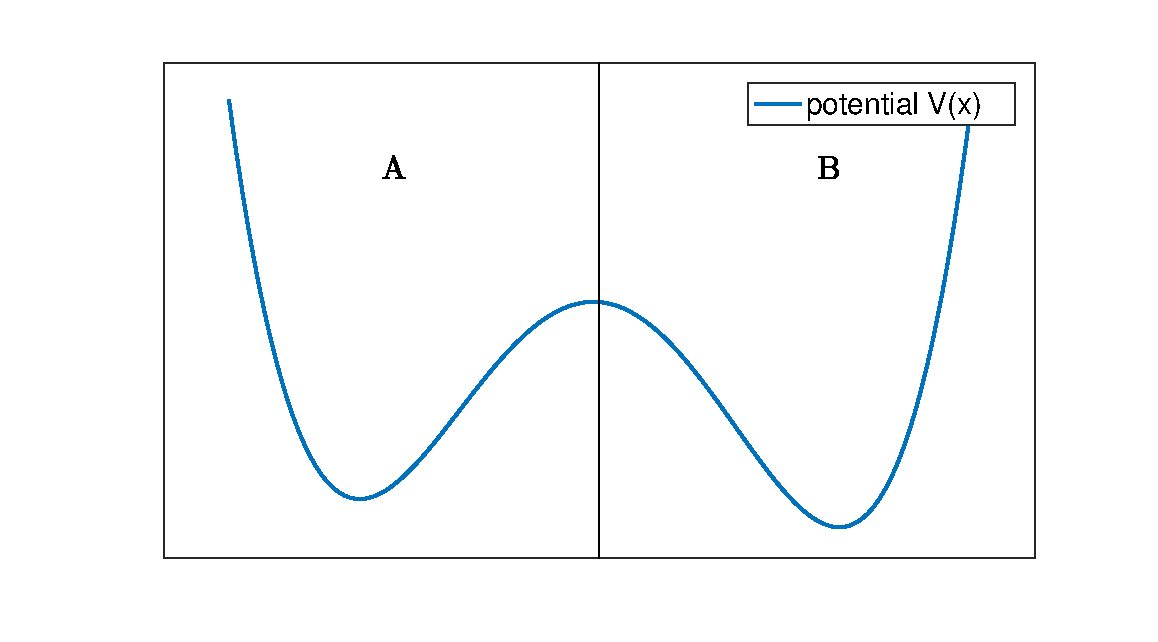
\includegraphics[width=0.6\textwidth]{figures/doublewell.eps} %70% der Textbreite
	\caption{Full-partition of a double-well potential}
	\label{fig:doublewell}
\end{figure}


For a small lag-time $\tau = 0.1$ we compute the probability of $\xtilde_k$ to make a transition from $B$ to $A$ in one time-step. We compare it to the probability of the same transition with the \textbf{additional} information of having been in $A$ one time-step before/earlier. If the process was Markovian, then this additional information about the past should make no difference and consequently, both probabilities should be equal.
We compute them in terms of the original process $X_t$ by
\begin{equation*}
\Prob_\mu[X_{(k+1)\tau} \in A \mid X_{k\tau} \in B] \textrm{ and }
\Prob_\mu[X_{(k+1)\tau} \in A \mid X_{k\tau} \in B, X_{(k-1)\tau} \in A].
\end{equation*}
Using the density functions $v_B$ and $v_{BA}$, we get %\marginpar{$v$ densities?}
\begin{equation}
\label{eq:recrossing1}
\Prob_\mu[X_{(k+1)\tau} \in A \mid X_{k\tau} \in B] = \int_A v_B^\tau(x) \diff x = ... ,
\end{equation}
\begin{equation}
\label{eq:recrossing2}
\Prob_\mu[X_{(k+1)\tau} \in A \mid X_{k\tau} \in B, X_{(k-1)\tau} \in A] = \int_A v_{BA}^\tau(x) \diff x = ... .
\end{equation}
We see that for such a short lag-time $\tau$, the process $\xtilde_k$ is \textbf{not} independent of the past  and hence \textbf{not} a Markov process.
%the process $\xtilde_k$ is \textbf{not} memoryless
%That behaviour is intuitively clear.
Equation \eqref{eq:recrossing1} describes the probability to get from $B$ to $A$, where ``being in $B$'' could mean everything from ``close to the transition region'' to ``far away from the transition region''. This probability is averaged over \textbf{all} possible starting points in $B$, since the spatial arrangement inside of $B$ is not included in this model. \marginpar{?} %specified/included
We compare it to \eqref{eq:recrossing2}, where being in $A$ shortly before
%immediately one time-step; moving to B
being in $B$ \textbf{increases} the probability to return to $A$ again. %return/recross
This behaviour can be interpreted such that for a short time after a \textbf{transition}, the process is likely to be still inside ot the \textbf{transition region}.
In our example, the transition region is the area close to the maximum of potential energy. Thus, there still is an increased probability to return to the previous state,
because of the spatial situation shortly after the transition. %area/region
\\

%transition between states = crossing the ``barrier'' between the states..

%the probability that the process is still in the transition region. And to get to $A$ from the transition region in $B$ is just more likely than from any other region inside $B$.
%favorable spatial situation?

This issue is called the \textit{recrossing effect}, since additional memory  leads to an increased probability to ``recross'' the energy barrier shortly after a transition. %(=energy maximum) %as in \eqref{eq:recrossing2}
On the other hand, if we choose a large lag-time, e.g. $\tau = 100$, then the past transition from $A$ to $B$ in \eqref{eq:recrossing2} took place a long time ago. In that case we do not know if the process is still in the critical transition region; during that long lag-time it could also have been gone anywhere else. %cannot certainly know
%That means that we could describe the memory effect of $\xtilde$ as a \textit{short-time memory}.
That means that the memory effect included in $\xtilde_k$ gets smaller for larger lag-times and consequently can be considered as a ``short-time memory''. %gets/becomes. accordingly/consequently

\subsubsection*{Comparison to Markov State Model}

After having observed the recrossing effect as a memory effect when projecting the time-series of a given continuous process onto a finite subspace, we want to compare that result to the corresponding \textit{Markov State Model}. %\marginpar{def MSM}

So far, we considered the process $\xtilde_k$ belonging to the operator $G(\Pcal^k)$, that is the projection of a time-series of the original process.
%Now, we want to consider the Markov State Model, i.e. the process $\xhat_k$ which is described by the operator $(G(\Pcal))^k$. The corresponding matrix representation is given by $P_c$ (see theorem \ref{thm:galerkin}).
Now, let $(\widehat{X}_k)_{k\in\mathbb{N}}$ be the Markov chain that is described by the transition matrix $P_c$, i.e. the matrix representation of the discretized transfer operator $G(\Pcal) := G\Pcal G$.
\\

A desirable behaviour of this model would be that $\widehat{X}_k$ and $\widetilde{X}_k$ have the same trajectory when started on the same initial distributions $\widehat{X}_0$ and $\widetilde{X}_0$. It will turn out that this is normally not the case. \marginpar{naja}
%Another desirable property would be Markovianity of both models, since this is the case for the original process $X_t$. But we have alredy seen in theorem \ref{thm:galerkin} that the matrix representation $P_c$ of $G\Pcal G$ is in general not a transition matrix, i.e. $\widehat{X}_k$ is not Markovian
%shown/visualized
This question is visualized in diagram \ref{fig:diagram_transfer}.
%Does it make a difference if we first project the process and then propagate it and vice versa?
Does it make a difference if we project the propagated process or if we propagate the projected process?

\begin{figure}[!ht]
	\centering
%	\begin{tikzcd}
%		\Pcal(\tau) \arrow{d}{proj.} \arrow{r}{\tau \rightarrow \tau k}    & (\Pcal(\tau))^k \arrow{d}{proj.} 			\\
%		P_c (\tau)   \arrow{r}{\tau \rightarrow \tau k}            &  (P_c(\tau))^k \\
%	\end{tikzcd}	
	\begin{tikzcd}
	 \Pcal(\tau) \arrow{d} \arrow{r}{\tau \rightarrow \tau k}    & (\Pcal(\tau))^k \arrow{d} 			\\
	 P_c (\tau)   \arrow{r}{\tau \rightarrow \tau k}            &  (P_c(\tau))^k \\
\end{tikzcd}
\caption{Projecting and propagating a transfer operator.}
\label{fig:diagram_transfer}
\end{figure}
In general, this diagram is \textbf{not} commuting and hence, in general we have
\begin{equation*}
(P_c)^k \neq (P^k)_c.
\end{equation*}

For the example of a full-partition discretization, we know from section \ref{sec:galerkin} that the resulting Markov State Model is a Markov chain.
Thus, the non-Markovian process $\widetilde{X}_k$ is modelled by a Markov chain $\widehat{X}_k$.
%Thus, we have a Markov chain $\xhat_k$ as a model for the non-Markovian process $\xtilde_k$, so it is clear that there is a discretization/iteration error.
That is also where the term Markov State Model comes from. 
%We describe the non-Markovian process $\widetilde{X}_k$ by a Markov chain $\widehat{X}_k$.

\subsubsection*{Discretization Error} %(Density Propagating Error/Iteration Error)
%discretization/ projection/ propagating error
The maximal possible error between the distributions of $\widetilde{X}_k$ and $\widehat{X}_k$ after $k$ time-steps is given by \marginpar{which norm?}
\begin{equation*}
E(k) = \Vert G(\Pcal^k) - (G (\Pcal))^k\Vert.
\end{equation*}
%independently of initial distribution

\begin{thm} %discrete/dominant spectrum. given/denoted/ordered
Let $\Pcal$ be a transfer operator with the dominant spectrum $1=\lambda_0 > \lambda_1 \geq \dots \geq \lambda_n$.
%Assume the dominant spectrum of a transfer operator $\Pcal$ is given by $1=\lambda_0 > \lambda_1 \geq \dots \geq \lambda_n$.
Then the projection error can be bounded from above in terms of the second-largest eigenvalue by
\begin{equation*}
\Vert (G (\Pcal))^k - \Pi_0\Vert \leq \lambda_1^k,
\end{equation*}
where $\Pi_0$ is the orthogonal projection of ... .
\end{thm}

For a proof, see Sch\"utte and Sarich\cite[p.72]{schutte2013metastability}.
%illuminating
In the next chapter we demonstrate the deep relation between the spectrum of the transfer operator and the long-time behaviour of the process. %further/deeper
%Furthermore, there is a relation between smallness of the  projection error and the metastability of a %subdivision of the state space.
%Schuette, Huisinga. Or Sarich p.58
%\marginpar{def MSM, $P_c$}
We will see how to choose a convenient basis for a MSM such that the iteration error vanishes, i.e. the long-time behaviour of the original process is preserved. \marginpar{?}
%approximation/iteration/discretization error

\subsubsection*{Conclusion}

%What is the recrossing effect??? That the process loses its Markovianity?
%Iteration Error = that there is a deviation %between project/propagate and propagate/project?

We have to distinguish between two kind of ``errors'' that can occur:
\begin{itemize}
\item Rebinding Events: Projection can include some kind of memory effect
\item Iteration Error: Deviation of $G(\Pcal^k)$ and $(G(\Pcal))^k$
\end{itemize}

%\chapter{Metastability and Dominant Structures}
\chapter{Dominant Structures in Markov Processes}\label{chap:meta}
% in Markov Processes
  %method/technique
With the Galerkin discretization, we introduced a method to reduce the dimension of a Markov process by projecting it onto a smaller state space.
However we don't know yet how to choose a partition of unity such that this projection yields a reasonable Markov State Model, in the sense that important properties of the original process are maintained.
%inherited,maintained
%by metastability, by a metastable behaviour, metastable sets
Usually, the long-time behaviour of a process is of particular interest. It is often determined by a so called metastable behaviour.
%It describes the typical behaviour of rare transitions between specific subsets, called \textit{metastable} or \textit{dominant subsets}, after a long duration of stay inside.
We will see why it makes sense to project a process onto its metastable sets and, in order to detect them, analyze their relation to the dominant spectrum of the transfer operator.
We will also see that the optimal metastable decomposition is not sharp/crisp but soft/fuzzy.
%in terms of membership functions

%introduce/present. decompose the state space/cluster a process/create a MSM
Additionally, with the aid of the Schur decomposition we introduce a rather new approach to create a Markov State Model. In contrast to the spectral approach, it includes nonreversible processes and is even able to identify further structures.
%cluster a broader class of processes.


\section{Metastability}
\label{sec:metastability}

There exist several definitions of metastability. %different definitions
%Shortly said, metastability is the property of a process that its state space consists of subsets/regions such that transitions between these subsets are rare events while the duration of stay inside of each of them is rather long.
Shortly said, metastability is the property of a process to act on particular regions such that transitions between these regions are rare events while the durations of stay inside of each of them is rather long.
%these subsets is rather long.
Some possible characterizations of that behaviour are based on large hitting times or small exit rates, see Sch\"utte and Sarich\cite[chapter 3]{schutte2013metastability},
where a good overview of the most common definitions can be found.
%which gives a good overview of the most common definitions.

\subsubsection*{Mathematical concept of metastability}

%define, introduce. $A \in \Sigma$?
In order to describe the concept of metastability, it is a good way to start with so called \textit{stable} or \textit{invariant subsets}. A measurable subset $A \subset E$ of the state space of a Markov process $X_t$ is called stable or invariant if it cannot be left, i.e. if $\Prob(X_t \in A \mid X_0 \in A) = 1$ for all $t$.
%Similarly
Analoguously, we can define a \textit{metastable} or \textit{almost invariant subset} as a subset in which the process will stay for a very long time before exiting it into any other subset, that is $\Prob(X_{t_f} \in A \mid X_0 \in A) \approx 1$ for a convenient timescale $t_f$.
%Metastability: A subset is not invariant but almost invariant
%Consequentially
Thus, a full partition $A_1,\dots,A_n$ of the state space $E$ is called \textit{metastable} if
\begin{equation}
\label{eq:metastability}
\sum_{k=1}^n \Prob_\mu(X_{t_f} \in A_k \mid X_0 \in A_k) \approx n.
\end{equation}
%mu??
Then each of the sets $A_k$ is almost invariant with respect to timescale $t_f$;
the probability to stay in one of the partition sets being started there is almost $1$, while the probability to change between any two different partition sets is almost $0$.
Such a partition is also called a \textit{metastable decomposition}.
%of the state space?

Obviously, being ``close to 1'' or ``close to $n$'' are rather vague statements.
However, that lack of concreteness will be eliminated later, since we will only be interested in the ``best'' metastable decomposition.
%That means that we want to obtain a decomposition where the sum \eqref{eq:metastability} is as close as possible to $m$, or equivalently the probability to stay inside of a metastable set is as close as possible to $1$.
%High holding probability?
That means that we want to obtain a decomposition where the probability to stay inside of each metastable set is as close as possible to $1$, resulting in the sum \eqref{eq:metastability} being as close as possible to $n$.
Likewise, the choice of the timescale $t_f$ is not specified in general and will depend on the particular system in consideration.
%has to be specified for each model individually. system/question in consideration/investigation/case
Hence, the only parameter in \eqref{eq:metastability} that has to be determined is the number $n$ of subsets we are looking for.
%\marginpar{joint metastability?}

\subsubsection*{Metastability in molecular systems}

Metastability is a very important concept for stochastic processes corresponding to molecular systems. Such processes describe the movement of atoms or molecules in space and
have the characteristic behaviour to oscillate or fluctuate around equilibrium positions on the smallest time scales (about one femtosecond). \marginpar{BM?}
In contrast to these fast oscillations, the process often stays inside of a certain region, called \textit{conformation}, for a long time before switching to another region (nano- or millisecond time scale).
%%switching/changing/exiting. region/subset. comparatively/relatively
Since transitions between conformations are relatively rare events, they can be identified as metastable sets if we choose a convenient timescale.
Such a behaviour is depicted in figure \ref{fig:conformations} on the example of the dihedral angle of a molecule, taken from Weber\cite{weber2011subspace}.

%\marginpar{conformation = spatial arrangement? special case of metastability?}
% long duration of stay + small transition rates/probabilities/ rare transitions between these subsets

\begin{figure}[!htb]
	\label{fig:conformations}
	\centering
	\includegraphics[width=0.7\textwidth]{conformations.jpg} %70% der Textbreite
	\caption{Example of a molecule with two (metastable) conformations. The dihedral angle of the molecule can take values between $+45^\circ$ and $-45^\circ$. There are two regions, highlighted red and blue, where the process stays for a rather long time and oscillates \textbf{inside}. Transition between these regions don't occur often. Thus, these two conformations can be identified as metastable sets.}
\end{figure}


%This dihedral angle can take values between $+45^\circ$ and $-45^\circ$.
%Thus, the process acts on a continuous state space and has infinitely many states.
%There are two regions, highlighted red and blue, where the process stays for a rather long time and oscillates \textbf{inside}.
%Transition between these regions don't occur often.
%and that transitions between these regions are rare.
%Thus, these two conformations can be identified as metastable sets.
%(metastable) conformations.

%useful
As transitions between metastable sets are rare events, long-time simulations of a process are required in order to get informations about conformational changes.
%%Thus, conformational changes are rare events and will show up only in long term simulations of the dynamics (nano- or millisecond time scale).
%complex systems
However long-time simulations of such large systems are not feasible in reasonable time even with the best computers nowaday, see Anton\cite{shaw2009millisecond} or its successor Anton$2$\cite{shaw2014anton}.
%supercomputers, designed for the purpose of such molecular dynamic simulations. %Unfortunately..

%needed/required
Hence, in order to be able to compute some long-time simulations of a given molecular system, a reduction of complexity  is needed. This can be achieved by a clustering of the state space via a Galerkin projection as depicted in section \ref{sec:galerkin}. Different states will be clustered appropriately such that we get a process on a smaller state space.
%depicted, described
\\

This point of view also motivates the following terminology. A state in the original state space is called a \textit{micro state}, as it is a state considered on the microscopic or atomistic level. In order to get a smaller state space, micro states are grouped together and such a cluster is called a \textit{macro state}, since we are now considering the process on a macroscopic level (cannot distinguish between smaller states/atoms anymore).

For instance, the spatial coordinates of a single atom could be considered as a micro state, while the corresponding macro state is a cluster of several atoms. If we are working on this smaller state space, we cannot distinguish anymore between the single atoms of the cluster (forget information).

\subsubsection*{Clustering into metastable sets}

%(i.e. how to choose the partition of unity for Galerkin projection)
%represents the correct long-time behaviour of the original process
The question \textbf{how} to cluster a given process such that it maintains the long-time behaviour of the original process can be answered easily with the following intuitive approach: As the long-time behaviour of a process is described by the metastability of the system, we choose the metastable sets as clustering sets.
%described, determined, based
More clearly, we create a new process where each macro state corresponds to one of the metastable sets.
In order to represent the correct long-time behaviour of the original process, the transition probabilities of the clustered process/reduced model should correspond to the transition rates between the metastable sets.
\\

%clusters/macro states/membership fcts.
%projected model

%cluster/group together
%As we are mainly interested in the long-time behaviour of a given process, it seems reasonable to cluster states of a metastable set together and create a new process where each macro state corresponds to one of the metastable sets. The transition probabilities of the clustered process/reduced model should correspond to the transition rates of the original process between its metastable sets. \marginpar{micro/macro states}
%between the macro states
%In order to..
%maintains, inherits, keeps
%determined in terms of
As metastability is determined on
%As metastability describes a behaviour on
%reduced model/projected process/clustered process
long timescales, the projected process maintains the long-time behaviour of the original process, but forgets about short-time transitions, i.e. transitions inside of a conformation/metastable set.

Since there is not one unique metastable decomposition of the state space, we need to find a decomposition which is in some sense ``the best''; then we can use it to create a reduced model. In the next sections we will see how to find such a decomposition.
\\

%clustering not unique: different metastable decompositions
%For example: in which metastable set should we assign a
%transition region (e.g. a region which is close to several metastable sets). SOLVED BY MEMBERSHIP?

%Going from micro states to macro states.

%\subsubsection*{Advantages / Disadvantages}

%projected/clustered
%reduced dimension/complexity
Most importantly, the clustered process will have the desired property of a reduced complexity since the model acts on a smaller state space.
%while maintaining the crucial property of the original process (transitions between metastable sets = long-time behaviour).
Therefore, the computation effort for long-time simulations is definitely decreased.
Furthermore, we get a better overview of the system, since it is always easier to consider a process on a few states in comparison to a process on a very large or even continuous state space.
However, it has to be guaranteed that the clustered process represents the \textbf{correct} long-time behaviour of the process. How this can be ensured will be explained in section \ref{sec:fuzzy}.
\clearpage
  \section{Spectral Approach}
\label{sec:spectral}

%connected,related
%In this section we show that the spectrum of the transfer operator is highly connected to the metastability of the corresponding Markov process.
In this section, we demonstrate the strong relation of the metastability of a Markov process to the spectrum of the associated transfer operator. %associated/corresponding
%spectrum of the transfer operator to the metastability of the corresponding Markov process.
More precisely, the existence of metastable sets implies the existence of dominant eigenvalues of the transfer operator and vice versa.
The idea to detect metastable sets via dominant eigenvalues has been first proposed by Dellnitz and Junge\cite{dellnitz1999approximation} and transferred to molecular dynamics by Sch\"utte et al\cite{schutte1998conformational,schutte1999direct}.

\subsubsection*{Existence of dominant eigenvalues}

%The \textit{multiplicity} of an eigenvalue $\lambda$ is defined as the dimension of the generalized %eigenspace. Eigenvalues of multiplicity $1$ are called  \textit{simple}.

%Let us, lag-time t
We consider the transfer operator $\Pcal := \Pcal(\tau)$ of a Markov process for some fixed lag-time $\tau$ in the Hilbert space $L^2(\mu)$. \marginpar{ $L^2$, $L^1$?}
%$L^1$ Huisinga diss; why $L^2$, $L^1$ enough?
%For further informations, see Kato\cite{kato1995}.
We are interested in \textit{dominant eigenvalues} of $\Pcal$, that is large eigenvalues which are close to 1 and separated from the rest of the spectrum.
The \textit{discrete spectrum} $\sigma_{\mathrm{discr}}(\Pcal)$ is the set consisting of all eigenvalues $\lambda \in \sigma(\Pcal)$ that are isolated and of finite multiplicity.
%contains all
The \textit{essential spectral radius} $r_{\mathrm{ess}}(\Pcal)$ is defined as
\begin{equation*}
r_{\mathrm{ess}}(\Pcal) = \inf \{ r \geq 0 \mid \lambda \in \sigma(\Pcal) \textrm{ with } |\lambda| > r \textrm{ implies } \lambda \in \sigma_{\mathrm{discr}}(\Pcal) \}.
\end{equation*}
%essential/continuous. under consideration
The existence of dominant eigenvalues requires that the continuous part of the spectrum is bounded away from the dominant elements of the discrete spectrum.
To ensure that the process we are considering actually possesses metastable sets, we need to pose some conditions on the spectrum of the transfer operator:
\begin{description}
    \item[C1] The essential spectral radius of $\Pcal$ is less than one, i.e. $r_{\mathrm{ess}} < 1$.
    \item[C2] The eigenvalue $\lambda=1$ of $\Pcal$ is simple and dominant, i.e.
    %i.e. $\eta \in \sigma(\Pcal)$ with $|\eta| = 1$ implies $\eta = 1$.
    \begin{equation*}
    \eta \in \sigma(\Pcal) \textrm{ with } |\eta| = 1 \textrm{ implies } \eta = 1.
    \end{equation*}
\end{description}
%criteria for it
We will not go into further details for which processes the two above conditions are fulfilled; some criteria can be found in Huisinga\cite[chapter $4$]{huisinga2001metastability}.
Since we are interested in a metastable behaviour, we assume that the processes under investigation satisfy these conditions.
%Since these conditions are required for the later investigations, we will just assume that they are true.
We need condition {\textbf{\textsf{C1}} to ensure that the continuous part of the spectrum is bounded away from the discrete eigenvalues. Otherwise they would not be dominant anymore and the process would be rather rapidly mixing than having any metastable sets.
%metastable sets/dominant structures
Condition {\textbf{\textsf{C2}} however is important because the state space of a transfer operator with more than one eigenvalue of absolute value $1$ can be decomposed into invariant sets, that is subsets which cannot be left. \marginpar{absolute?}
%\marginpar{C2 = ergodic?}
%\marginpar{has periodic structures?}
%stable/invariant
However, such a case is not interesting for us.
%\marginpar{excludes modeling and interpretation problems}
Instead, we want to know more about \textbf{almost} invariant sets and their critical transition regions. 
%We will consider only ergodic process which means theat the eigenvalue $1$ is unique.
\\


%transfer operator for a process unique?
The transfer operator $\Pcal: L^2(\mu) \rightarrow L^2(\mu)$ of a reversible process satisfying the properties \textrm{\textbf{\textsf{C1}}} and \textrm{\textbf{\textsf{C2}}} is self-adjoint by theorem \ref{thm:selfadjoint_reversible} and has a spectrum of the form
%has a spectrum of the form/the following spectrum
%\marginpar{why discr. rechts?}
\begin{equation*}
\sigma(\Pcal) \subset [a,b] \cup \{\lambda_n\} \cup \dots \cup \{\lambda_2 \} \cup \{1\}
\end{equation*}
with $-1 < a \leq b < \lambda_n \leq \dots < \lambda_1 = 1$ and isolated, not necessarily simple eigenvalues of finite multiplicity that are counted according to multiplicity.


\subsubsection*{Relation of dominant spectrum to metastability}

%state,determine
In order to find out about the quality of an arbitrary decomposition, we present upper and lower bounds for the metastability of the decomposition in terms of dominant eigenvalues and eigenvectors of the transfer operator.
We will denote by \textit{metastability of a decomposition $\Dcal$} the sum of the metastability of its subsets.

%Sch\"utte\cite[theorem 4.16]{schutte2013metastability}
\begin{thm}[{Huisinga and Schmidt\cite[Theorem 2.4]{huisinga2006metastability}}]
\label{thm:metastability_bounds_1}
Let $\Pcal$ be the transfer operator of a reversible process satisfying \textrm{\textbf{\textsf{C1}}} and \textrm{\textbf{\textsf{C2}}}.
Let $\lambda_1,\dots,\lambda_n$ denote its isolated eigenvalues and $v_1,\dots,v_n$ the corresponding eigenfunctions, normalized to $\Vert v_i \Vert_2 = 1$.
Let $Q$ be the orthogonal projection of $L^2(\mu)$ onto $\mathrm{span}\{\eins_{A_1},\dots, \eins_{A_n}\}$.
The metastability of an arbitrary decomposition $\Dcal = \{A_1,\dots, A_n\}$ of the state space $E$ can be bounded from above by
\begin{equation*}
p(A_1,A_1) + \dots + p(A_n, A_n) \leq 1+ \lambda_2 + \dots + \lambda_n,
\end{equation*}
while it is bounded from below by
\begin{equation*}
1+ \rho_2 \lambda_2 + \dots + \rho_n \lambda_n + c \leq p(A_1,A_1) + \dots + p(A_n, A_n),
\end{equation*}
where $\rho_j = \Vert Q v_j \Vert_{L^2(\mu)}^2 = \langle Qv_j, Qv_j \rangle \in [0,1]$ and $c = a(1-\rho_1) \cdots (1 - \rho_n)$.
\end{thm}

%shows,reveals. relation/connection. eigenfunctions and eigenvalues
Theorem \ref{thm:metastability_bounds_1} reveals the strong relation between metastable sets and the dominant eigenvalues of the transfer operator.
%enables,allows,provides us an insight into. evaluate,judge,rate
It allows us to evaluate the quality of a decomposition by comparing the lower and the upper bound of metastability.
The upper bound shows that eigenvalues far away from $1$ worsen the metastability of a decomposition.
The lower bound is close to the upper bound if the dominant eigenfunctions $v_2,\dots,v_n$ are almost constant on the metastable subsets $A_1,\dots,A_n$, implying $\rho_j \approx 1$ and $c \approx 0$.
Moreover, Huisinga and Schmidt\cite{huisinga2006metastability} show that the lower and upper bounds from theorem \ref{thm:metastability_bounds_1} are sharp and asymptotically exact.

That provokes the question if there exists an \textbf{optimal} decomposition with the highest possible metastability. \marginpar{maybe ill-conditioned}
%In fact, this problem might unfortunately be ill-conditioned.
By all means, this theorem indicates that the number of metastable sets should be determined by the number of dominant eigenvalues.
\\

Deuflhard et al\cite{deuflhard2000identification} proposed an algorithm to identify the metastable sets of a Markov chain by exploiting the sign structure of the dominant eigenvectors of the transition matrix.
\\

In figure \ref{fig:spectrum}, we get a good overview of the relation between the eigenfunctions of the transfer operator and the metastable sets of the corresponding process. We have a potential/energy landscape with 4 energy minima, that is 4 regions where the process could be \textit{trapped} such that it is hard to get outside again. The transition matrix  shows this metastable behaviour since we can see 4 regions which large probabilities to stay inside and very small probabilities to go to a different region.
Furthermore we see that the process has 4 dominant eigenvalues. Three of them have a change of sign, inducing a metastable decomposition.
\newpage


\begin{figure}[!ht]
	\label{fig:spectrum}
	\centering
	\subfigure[Transition matrix $P$ on $100$ states with $4$ visible metastable sets]{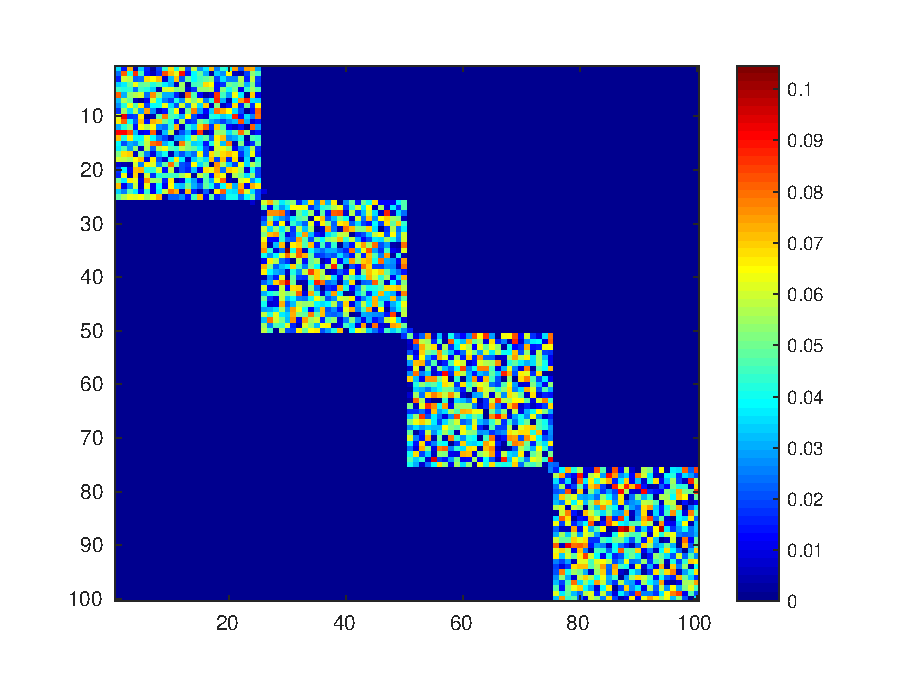
\includegraphics[width=0.49\textwidth]{figures/spectral/transition.eps}}
	\subfigure[Spectrum of $P$ with $4$ dominant eigenvalues]{\includegraphics[width=0.49\textwidth]{figures/spectral/eigenvalues.eps}}
	\subfigure[Dominant eigenvectors of $P$ with change of signs corresponding to the transition regions]{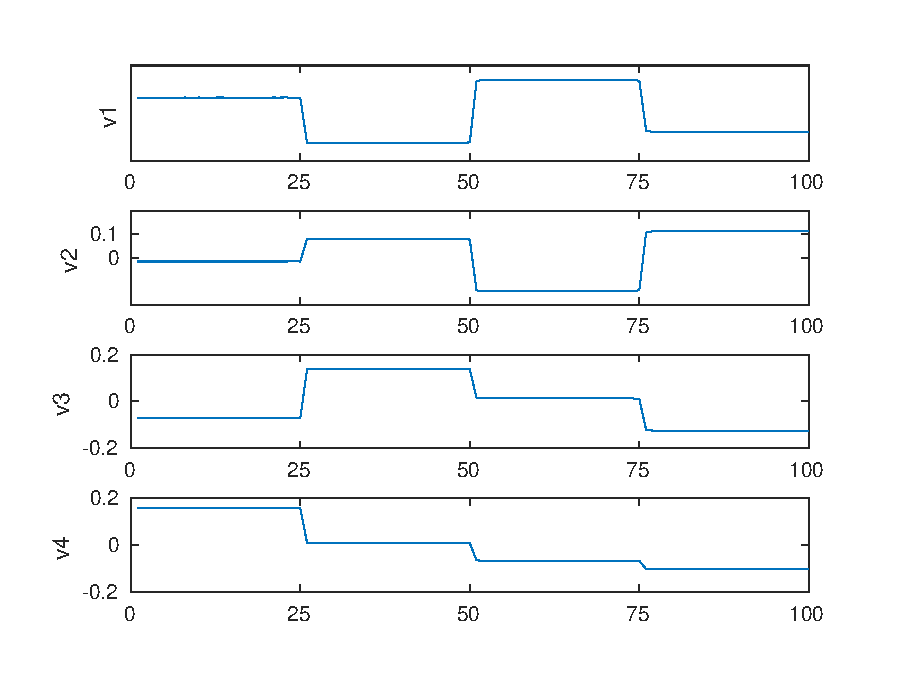
\includegraphics[width=0.49\textwidth]{figures/spectral/eigenvectors.eps}}
	\caption{Relation of the transition matrix to its spectrum with regard to metastability}
\end{figure}

%anschaulich
%This theorem gives us a first demonstrative relation of the metastability of a process to its eigenvectors. This %result is not yet optimal/very good. In the next sections, we will see that linear combinations of eigenvectors %result in much better metastability.


This relation can be explained as follows.
A process consisting of $n$ invariant sets $\{A_1,\dots,A_n\}$ has the $n$-fold eigenvalue $1$ and the corresponding eigenvectors $\eins_{A_i}$ are constant on the invariant sets.
A metastable process consists of almost invariant sets and thus, can be interpreted as the perturbation of a process with invariant sets, by introducing small transitions between the invariant sets. Accordingly, the eigenvalues and eigenvectors are perturbed. This results in one eigenvalue $1$ and $n-1$ eigenvalues close to $1$, having eigenvectors that are almost constant on the almost invariant sets.
A detailed perturbation analysis can be found in Deuflhard et al\cite{deuflhard2000identification}.

\subsubsection*{Disadvantages}
%Conclusion
%Advantages, Alternatives

%suitable,convenient
%to characterize metastability of Markov processes, respectively. wrt its metastable sets
%convenient,suitable,possible,feasible
The spectral approach is an appropriate method to cluster a process with respect to metastability, though it bears some disadvantages.
%1:
The result is only appliable on reversible processes, because real eigenvalues are only guaranteed if the transfer operator is self-adjoint. \marginpar{see}
%2:
%Moreover, the eigenvector problem of the transfer operator has only global solutions. \marginpar{global = good?}
%Most of all,
Particularly, the previous procedure to compute a metastable decomposition does not take into consideration the existence of transition regions.
This can lead to an iteration error, i.e. the clustered process does not represent the correct long-time behaviour.
%needs refinement/improvement
\\

%clarify/point out/emphasize/highlight
This section has been presented mainly with the aim to emphasize the strong relation of the spectrum of the transfer operator to the metastability of the system. %mainly/merely/solely/only
%results in a full partition decomposition and
However, this approach does \textbf{not} represent the state of the art.
%This relation can be seen best for a full partition decomposition/clustering.
%enhanced/improved. related, but improved,
In the next section, we deduce an enhanced method, resulting in a \textbf{soft} clustering instead of a full partition decomposition.
%, which likewise takes advantage of this strong relation between spectrum and metastability.
%It also includes the eigenvalues and eigenfunctions of the transfer operator, but will be soft instead of crisp.
%comprises/includes the eigenvalues and eigenfunctions of the transfer operator, but it will be fuzzy.

  \section{Fuzzy Clustering}
\label{sec:fuzzy}

%(metastable decomposition induced by zeros of eigenfunctions)
The above considerations result in a metastable full decomposition of the state space, that is each state is assigned to exactly one of the partition sets.
We will see now, that there exist better solutions, considering/including the fact that transition regions can belong to several metastable conformations. So for this slightly more general approach,
%(already examined/investigated/analyzed in recent research, see  ...),
there may be some overlap in the assignment of states to metastable sets.

% a transition region can be %assigned to several macro states with different weight(?).

\subsubsection*{Set-based vs. Function-based Approach}
An intuitive approach to decompose the state space would be to determine a certain number of metastable sets which form a full partition of the state space, such that each state is assigned to exactly one of the metastable sets.
%each partition corresponds to one conformation/ metastable set.
The problem with that approach is that also the transition regions of the process would have to be assigned to one of these partition sets. But why would you assign a state in a transition region to one adjacent metastable set and not to the/one other? So such an assignment is not a rigoruous description of actual behaviour of the process.
%does not make so much sense.

Therefore, this \textit{set-based} or \textit{crisp approach} of decomposing the process has been replaced by the \textit{function-based} or \textit{fuzzy/soft approach}.
That means that each state of the process is assigned with a certain ``degree of membership'' ($\approx$ probability) to each metastable conformation.
That is reasonable, because a state in a transition region (local minimum) cannot be assigned to a single conformation. Thus, these clustering-functions should be ``overlapping''.
%allowing to assign a state to different conformation with certain probabilities/degree of membership

\begin{figure}[!ht]
	\centering
	\includegraphics[width=0.5\textwidth]{figures/fig_fuzzy_set.jpg}
 	\caption{Crisp vs Fuzzy Sets/ Clustering}
        \label{fig:fuzzy}
\end{figure}

%\subsubsection*{Fuzzy Sets}

Fuzzy sets are sets whose elements have degrees of membership.

%\begin{defi}[Fuzzy Set]
%A fuzzy set is a pair $(U,m)$ where $U$ is a set and $m:U \rightarrow [0,1]$ a membership function.
%\end{defi}

\subsubsection*{Membership functions}

%reversible
Assuming we have already determined that our process consists of $n$ metastable sets (by knowing its $n$ dominant eigenvalues).
%the number of metastable sets by 
%we are considering a stochastic process with $n$ dominant eigenvalues
We will follow the approach of Weber\cite{weber2006meshless} to define macro states as \textit{overlapping partial densities}. They can be identified by membership functions $\cfam : \X \rightarrow [0,1]$. Each state of the original state space shall be assigned to the different macro states with a certain \textit{degree of membership}.
%using membership functions (linear combinations of eigenfunctions). no??

\begin{defi}[Membership Function \cite{weber2006meshless}]
% (see \ref{sec:galerkin})
The functions $\cfam : \X \rightarrow [0,1]$ are called \textit{membership functions} if they fulfill
\begin{itemize}
\item $\chi_j(i) \geq 0$ $\forall i \in \X$ and $\forall j \in \{1,\dots,n\}$ (positivity),
\item $\sum_{j = 1}^n \chi_j(i) = 1$ $\forall i \in \X$ (partition of unity).
\end{itemize}

%For any set $\X$, a membership function on $\X$ is a function $m: \X \rightarrow [0,1]$.
%A membership function is a function $\chi_i : \X \rightarrow [0,1]$ \marginpar{part. of unity?}
%= partition of unity and nonnegative
\end{defi}

%finite state space: membership vectors (for PCCA+ since we can only apply it on finite processes?)
We can interpret membership functions as assigning each state $i$ to a cluster/conformation $j$ with a certain ``probability'' $\chi_j(i)$.
%or ``degree of membership''
For each conformation $j \in \{ 1 , \dots, n \}$, there is a membership function $\chi_j$, which determines the portion of the partial density w.r.t. the total density function. \marginpar{?}
These membership functions form a partition of unity, in order to sum up to the total density.
%some density function given? t.ex. Boltzmann distribution
%Weber Diss 10
\\

The previous example of a full-partition discretization corresponds to the choice of characteristic functions $\{ \eins_{A_1},\dots, \eins_{A_n} \}$ as membership functions. They are also called \textit{crisp} or \textit{hard} membership functions, whereas the general (overlapping) membership functions are denoted as \textit{fuzzy} or \textit{soft}.
%while/whereas
The \textit{crispness} of the clustering(?) can be measured by the matrix $S$.
Nonoverlapping membership functions (char. fcts.) yield an overlap matrix $S = D\inv \langle \chi, \chi \rangle$ equal to the unit matrix.
Overlapping membership functions yield a matrix with non-zero outer diagonal elements.
\\

Membership functions can be used to decompose the space into metastable sets/clusters. In this case, the assignment of a state to a metastable set must not be unique, but a state can belong to different metastable sets with certain degrees, which can be interpreted as kind of probabilities. \marginpar{?} That model takes into consideration
%takes into account
the existence of transitions regions which cannot be uniquely assigned to one macro state/metastable set.
%detect a 

%membership functions: continuous and overlapping

Since membership functions form a partition of unity, we can apply the Galerkin projection as defined in section \ref{sec:galerkin}.
If we choose the membership functions w.r.t. metastability, then we get a Markov State Model where each (macro) state is a metastable set of the original process. \marginpar{so far: membership fct indep. of metast. set}
%As membership functions are a partition of unity, we can 1) create a metastable decomposition (maybe with %overlap, so no partition) and 2) apply Galerkin Projection on it (partition of unity necessary).
\\

Individual eigenfunctions $\Xcal$ do not overlap since they are orthogonal. But the membership functions $\chi_j$ as linear combinations of the dominant eigenfunctions might have an overlap.
 \marginpar{?}
\begin{equation*}
P_c \chi_j \approx \chi_j \ \forall j=1,\dots,n.
\end{equation*}
\begin{equation*}
T\chi_j \approx S\chi_j \ \forall j=1,\dots,n.
\end{equation*}

From the definition, membership functions like $\chi_1 = \chi_2 = 0.5$ are possible, but not interesting. Instead, they are often chosen to be \textbf{close} to a characteristic function, like shown in figure \ref{fig:fuzzy}. That is reasonable, since it puts the emphasis of a conformation onto a certain region (high degree of membership) and maybe some adjacent parts (low degree of membership).
For this reason, they are also often called \textit{almost characteristic functions} in literature.

\subsubsection*{Statistical Weights} \marginpar{what for?}

For each macrostate we can define a statistical weight
\begin{equation*}
w_i = \langle \chi_i, \eins \rangle_\mu = \int_\X \chi_i(q) \diff \mu(q),
\end{equation*}
which describes the \textit{portion} of a membership function to the total density function. \marginpar{?}
$D = \mathrm{diag}(w_1,\dots,w_n)$ is the diagonal matrix of the statistical weights of the membership functions. Then $T=D^{-1} \langle \chi, \Pcal(\tau) \chi \rangle_\mu$, compare theorem \ref{thm:galerkin}.

\subsubsection*{Perron Cluster Analysis} \marginpar{finite/cont. vec./fct.}

The term \textit{Perron Cluster Analysis} denotes the objective of clustering a Markov process into metastable sets using the \textit{Perron eigenvalues} respective \textit{Perron eigenfunctions}, which means eigenvalues close to $1$ and the corresponding eigenfunctions.
Perron Cluster Analysis respectively its algorithmic implementation PCCA (\textit{Perron Cluster Cluster Analysis}) has been developed by Deuflhard et al\cite{deuflhard2000identification} which used the sign structure of the dominant eigenvalues of the transition matrix. \marginpar{set-based approach?}
%as what?
That approach has been improved by Deuflhard and Weber\cite{deuflhard2005robust}
%\marginpar{oder Weber und Galliat?}
who transformed the system of eigenvectors into a system of membership functions which results in a soft/fuzzy clustering of the state space of the original process; their algorithm is called PCCA+
(\textit{Robust Perron Cluster Analysis}).
%adapted
Originally, PCCA+ was formulated only for discrete Markov chains, but Weber\cite{weber2011subspace} extended it even on continuous processes.
%we present here the more general case for cont. processes with a given transfer operator
\\

%The  whole approach  is  called Perron  cluster  analysis, its agorithmic  realization is  abbreviated  as  PCCA  %(from  Perron  Cluster  Cluster  Analysis). \marginpar{PCCA+: robust}
%We need to choose/determine convenient/suitable membership functions s.t. the metastable decomposition %becomes as good as possible. Normed eigenfunctions are one possibility (no overlap). But better: linear %combinations of eigenfunctions. \marginpar{only for finite matrices? or also cont. operator w/ eigenfct.?}

%Let $\Xcal$ be the eigenvector matrix, \marginpar{eigenfct.?} i.e. the $i$-th column of $\Xcal$ is an %eigenvector corresponding to the eigenvalue $\lambda_i$. \marginpar{only dom. spec.}

We consider the set of dominant eigenvalues $\{\lfam\}$ with the corresponding set of eigenfunctions $\Xcal = \{\xfam\}$.
They fulfill the eigenvalue problem $\Pcal(\tau) \Xcal = \Xcal \Lambda$ of the transfer operator $\Pcal(\tau)$, where $\Lambda = \mathrm{diag}(\lfam)$.
The set of membership functions $\chi= \{\cfam \}$ can be built as a linear combination $\Xcal \Acal$ of the dominant eigenfunctions, that is
\begin{equation}
\chi_j(q) = \sum_{i=1}^n \Acal_{ij} \Xcal_i(q), \ j=1,\dots,n.
\end{equation}
Here,  $\Acal = \{\Acal_{ij}\}_{i,j=1,\dots,n} \in \R^{n\times n}$ is a real matrix which should be chosen in such a way that the resulting membership functions fulfill the required properties/constraints; i.e. positivity and partition of unity.
%Noe Lecture 4 (MSM 2015) 
There are infinitely many transformations $\Acal$ of the eigenvectors resulting in a soft membership matrix
$\chi$ satisfying the positivity and partition of unity constraints.
Consequently, we have to determine the transformation  $\Acal$ that satisfies some optimality condition.
The algorithm PCCA+ computes the matrix $\Acal$ as the solution of a convex maximization problem, see Weber\cite{weber2006meshless}. \marginpar{optimal metastability?}
%yields
%In order to fulfill the partition of unity property of each $\chi_i$, the matrix $A$ has to be chosen s.t. $\chi$ %is row-stochastic.

\marginpar{only conv. lin.comb.?}
Weber shows in \cite{weber2011subspace} that the for choice $\chi = \Xcal \Acal$ (any linear combination of the eigenfunctions $\Xcal$), the discretization error of the Galerkin projection vanishes and hence, diagram \ref{fig:diagram_transfer} commutes. In particular, such membership functions preserve the Markov property of the process.
%preserves the Markov property of the process. \marginpar{even: discretiz. error vanishes}
%Markovianity
\\

If we project a finite process, then the above formulation results in a \textit{membership vector matrix} $\chi$, which is the result of a linear combination of the \textit{eigenvector matrix}.

\subsubsection*{Measuring/Maximizing crispness of }
%Weber Diss 58
The \textit{crispness} of .. can be measured by the matrix $S$.

The metastability of a process is defined via the trace of $P_c$, but can also measured via its determinant.
\marginpar{see ...}
If the metastability is high, then $\det(P_c)$ is close to $1$. More clearly, by multiplication of the determinant we have
\begin{equation*}
\det(P_c) = \det(S) \det(\Lambda).
\end{equation*}
Thus, in order to increase the metastability of a system, both determinants need to be high. $\det(S)$ is maximized if the linear combination $\chi = \Xcal \Acal$ is as \textit{crisp} as possible.
%maximize $\det(S)$

%\subsubsection*{Iteration Error}

%Second largest eigenvalue results in the best decomposition and so on ...

%But Better: linear combination of eigenfunctions (might have an overlap) (membership functions, PCCA+).
%That will be described more in the next subsection 2.4 where, in aim to get a really good MSM, we try to %find the best possible decomposition (?) into metastable sets (? not a partition anymore) 

%Do we need PCCA+ to find the best(?) membership functions. And with the help of these membership %functions we can apply a Galerkin Projection?
  \section{Dominant cycles (non reversible NESS process)}

\subsubsection*{Approaches for nonreversible processes}
What is the dominant structure of a nonreversible process? cycle?
What is egentligen the problem with nonreversible processes? non-real eigenvalues
\\

How can the computation of dominant cycles help to detect metastable sets/ metastables cycles?
\\

What is a metastable cycle?
\\

Definition dominant cycle

\subsubsection*{Schur Decomposition}
%[djur] chap 5
%same as PCCA+ but for nonreversible processes, so with Schur vectors instead of eigenvectors
Dominant structures will be defined utilizing the dominant Schur vectors
of the transition matrix instead of its eigenvectors.

A membership matrix can be defined as a linear combination of these Schur vectors.

\chapter{Rebinding Effect in a Given Kinetics}\label{chap:rebinding}
  In this chapter we are going to examine a special type of molecular dynamic systems, namely receptor-ligand systems.
To describe these systems rigorously we can use all the mathematical concepts/objects defined in the previous chapters.

To give a short overview about what is going to happen here. The kinetics of a molecular system can be described via a differential equation. The solution of this \marginpar{nop} differential equation is a Markov(?) process which can be described via a transfer operator (section \ref{sec:transfer}). This operator will be projected onto a finite-dimensional state space (section \ref{sec:galerkin}) which may spoil the Markov Property of the process (section \ref{sec:recrossing}). \marginpar{optimization}
%complies with
%mathematically based
This chapter is mainly based on Weber and Fackeldey\cite{weber2014}.
%also\cite{weber2012}?

%Here we will try to tackle this subject for nonreversible (NESS) processes also.

\todo{which model? Hamiltonian ($\Gamma$)? Hamiltonian w/ randomized momentum ($\Omega$ w/ any momentum)? Langevin? Diffusion Dynamics?}
%\todo{Ensemble}

\section{Receptor-Ligand System}

We will present the \textit{receptor-ligand-system} as particular molecular dynamic system and describe it mathematically using a differential equation.
We will discuss the so called \textit{Rebinding Effect} and set in in relation to the Recrossing effect known from section \ref{sec:recrossing}.
%merged/set together
%outlook for later/further investigations
As an outlook/motivation, we will explain how these two concepts can be set together in the important application of \textit{drug design} and how the rebinding effect can help to improve the effect/efficiency of drugs.
%an important application of the rebinding effect in such a receptor-ligand-system.

\subsubsection*{What is a MD system? Molecular Dynamics vs Kinetics} \marginpar{Weber p.10}
In the previous chapters, we have often mentioned molecular dynamic systems (MD systems) and some of their properties without actually explaining what such a system is.
A \textit{molecular system} consists of atoms that are connected by \textit{covalent bonds}. bla bla.
The potential energy function, or \textit{energy landscape}, of a molecular system results in a dynamical behaviour on different timescales.
The fastest timescales (vibrations of covalent bonds) are around $10^{-15}$ seconds. \marginpar{see ..}
bla. up to nanoseconds or, for protein folding, up to microseconds or seconds or even longer..

\subsubsection*{What is a Receptor-Ligand system?}

A receptor can be a protein or blabla. As we are mainly interested in the mathematical description of a system, we will not specify further, which kind of biochemic/molecular receptor we are considering. Instead for us, a receptor will just be an \textit{object} to which a ligand can bind.
%and thus prevents the receptor to bind to any other object/ligand. Ligand takes a degree of freedom away

A \textit{receptor} is (in general) a proteine molecule.
A molecule that binds to a receptor is called a \textit{ligand}.
Each receptor will only bind with ligands of a particular structure.
%lock-key

Ligand binding is an (chemical) equilibrium process, i.e. the reaction rates of the forward and backward reactions are equal. That means that the concentrations of the reactants and the products are constant
%doesn't change
(\textit{dynamic equilibrium}). \marginpar{see ..}

A ligand (L) can bind to a receptor (R) and form a receptor-ligand complex (LR) which can dissolve again into its two original components. These reactions can be represented in the following form
%can be described by the 2-state process
\begin{equation*}
\label{eq:reaction}
L + R \rightleftharpoons LR,
\end{equation*}
%representing the law of mass action?
which corresponds to the law of mass action. \marginpar{see ..}
The dissociation constant $k_d$
%is an equilibrium constant that ...: \marginpar{what is that?}
\begin{equation*}
k_d = \frac{[L] \cdot [R]}{[LR]},
\end{equation*}
where $[L], [R]$ and $[LR]$ are the concentrations of $(L),(R)$ and $(LR)$, respectively. This constant is commonly used to describe the affinity between a ligand $(L)$ and a protein $(P)$, i.e. how strongly/tightly the ligand can bind to his particular protein/receptor. If the dissociation constant is small, then there is a high binding affinity between the ligand and the receptor.
%Affinity is a measure of the tendency of a ligand to bind to its receptor. Efficacy is the measure of the bound %ligand to activate its receptor.
%Affinity: The ability of a drug to combine with a receptor to create a drug-receptor complex.
%Efficacy: The ability of a drug-receptor complex to initiate a response.
The association constant $k_a$ is just the inverse of the dissociation constant
\begin{equation*}
k_a = \frac{[LR]}{[L] \cdot [R]}.
\end{equation*}
There are different factors which can lead to a high or low \textit{binding affinity}. \marginpar{which?}
%like thermodynamical reasons, ... .

\subsubsection*{Bivalent Ligand}

Bivalent ligands consists of two (drug-like?) molecules connected by an (inert?) linker.

\subsubsection*{Mathematical Description of Receptor-Ligand-System}

Starting from the reaction equation \eqref{eq:reaction}, we can deduce that the ligand can be found in two different (macro) states: ``unbound'' $(L)$ or ``bound'' $(LR)$. Then the probabilities of the ligand to be in one of these states can be described by the probability vector $x^T = \frac{1}{s}(([L],[LR]))$, where $s = [L] + [LR] = \textrm{const.}$.
This leads to an ordinary differential equation
\begin{equation*}
\dot{x}^T = x^T Q_c.
\end{equation*}
The matrix $Q_c$ consists of the rates of reaction,
\begin{equation*}
Q_c = 
\begin{pmatrix}
-k_a[R] & k_a[R]  \\
k_d      & -k_d
\end{pmatrix},
\end{equation*}
where $k_a$ and $k_d$ are the association and dissociation constants. Thus, it is the transition rate matrix corresponding to a Markov chain, i.e. it describes a memoryless process.

We will later see that this mathematical description of a receptor-ligand-system is not accurate, since in fact, such a process \textit{will} have some kind of memory.

%\section{Rebinding Effect and Drug Design}
\marginpar{impact of multivalency on rebinding effect (Weber, Chem.)}

\subsubsection*{Rebinding Effect}

The rebinding effect has been characterized as a memory effect which leads to an additional thermodynamic weight of the bound state.
%Weber quantifying rebinding effect
%occurs when projecting a MD process onto a finite subspace??

In fact, a stochastic process describing a receptor-ligand molecular system is NOT necessarily Markovian. The Markovianity can be spoiled by the Rebinding Effect. If a Receptor-Ligand system dissolves, due to the favorable spatial situation (?) it is more likely to rebind again than to stay dissolved. %\marginpar{Zusammenhang zum Absatz davor?}

There are several papers (...) describing the rebinding effect from a chemical and a mathematical point of view. In chemistry, there are several reasons/factors for the rebinding effect discussed.

The rebinding effect has recently (...) been discussed to increase the binding affinity of a process.
\marginpar{?}

\subsubsection*{Relation to Recrossing Effect}
We remember that we described the recrossing effect in section \ref{sec:recrossing}. There, we also had a process on macro states described by a transition matrix and thus being a Markov chain. But in reality, the (clustered) process was not memoryless.
The same phenomena occurs with the rebinding effect. We have a transition matrix, even though our process has a memory. We want to quantify this effect.

\subsubsection*{Basics of Drug Design}
%inventive process of finding new medications
The term \textit{drug design} describes the development of new medications based on the knowledge of a
%Most commonly,
biological target. The drug is often a small molecule which can bind to a protein molecule (target/disease/receptor) and thus activates or inhibits its function (disease modifying). So drug design is basically about designing a molecule which is
%complementary to the binding site of target
complementary in shape and charge to the biomolecular target and therefore will bind to it, see Str{\o}mgaard et al\cite{stromgaard2002}.
%is about developing
More precisely, drug design describes the design of ligands, i.e. molecules that will bind tightly to the given target, see Tollenaere\cite{tollenaere1996}.
%target = receptor; drug = ligand.. simplified model
%disease: have a bad molecule/protein/receptor which can bind to a human cell and create sickness.
%in order to avoid sickness: want a drug/medicament/ molecule which binds to the disease, s.t.
%it is not possible to bind to the human anymore :)

%The most fundamental goal in drug design is to predict whether a given molecule will bind to a target and if %so how strongly.
%tendency to bind

In order to be an efficient drug, we aim/wish for a a high \textit{binding affinity}, which is a measure of the strength of the chemical bond.
That means that the designed ligands should easily bind to the receptors, remain in a binding or rebind quickly after being dissolved. If the binding affinity of a drug is too low, a higher concentration of the drug is needed instead,
%in order to be effective,
which is undesired because of possible side effects.
There are many factors that influence/affect the binding affinity of a drug/ligand, such as ... .
The rebinding effect has been recently investigated to increase the binding affinity of a ligand, mathematically described by Weber et al\cite{weber2012, weber2014} as well as chemically by e.g. Vauqelin\cite{vauquelin2010}. This effect will be examined in this thesis. As a \textit{high} rebinding effect is aimed/wished, we will derive a lower bound for this effect, i.e. we will \textit{minimize} it.
%several factors for high binding affinity: like good shape, multivalency

\subsubsection*{Drug Design}

An important application of receptor-ligand processes is drug design. In short: A drug consists of ligands which should bind to the receptors of the virus. If the drug creates many bindings, the virus is "bound" and cannot attack the human (cell?) anymore. Thus, many bindings are a favorable thing. So a high rebinding effect enhances the (overall?) binding affinity of the process/ system which is good for the efficiency of a drug. We want a high rebinding effect.
So in this chapter, we examine the minimal rebinding effect for a given Kinetics.
This task has been solved by Weber and Fackeldey\cite{weber2014} for reversible processes.
\marginpar{How: from bound to unbound}
  \section{Molecular Kinetics as a Projection}
\label{sec:projection}
\marginpar{Mol. Kinetics Weber p.10}

% deduce/develop/derive two different point of views 
In this section, we will basically embed the mathematical concepts/results of chapter \ref{chap:markov} into a chemical/physical context in order to get a rigorous description of molecular (dynamic/kinetic?) systems. In considering such systems, we can distinguish between two point of views: we will see how we can get from the \textit{atomistic (=microsopic)} to a  \textit{macroscopic} scale/point of view by a projection.

\subsubsection*{Micro States}
%Boltzmann distribution = example for a canonical ensemble
A micro state of a molecular system with $N$ atoms can be represented in a $6N$-dimensional \textit{phase space} $\Gamma = \Omega \times \Rdrei$, \marginpar{spatial/position space}
consisting of the \textit{configurational space} $\Omega = \Rdrei$ and the \textit{momentum space} $\Rdrei$. In the following, we consider systems in \textit{thermodynamical equilibrium}.
%assume equilibrium
%\R_{+}
One possible model is given by the \textit{Boltzmann distribution} $\pi: \Omega \times \R^{3N} \rightarrow \R$, a
\marginpar{prob. dens. fct.?}
probability distribution assigning to each micro state a probability depending on its energy and temperature,
see McQuarrie\cite{mcquarrie2000}. It can be expressed as
% in the form
\begin{equation}
%\pi(q,p) \propto \exp{(-\beta H(q,p))},
\pi(q,p) = \frac{1}{Z} \exp{(-\beta H(q,p))},
\end{equation}
%The distribution shows that states with lower energy will always have a higher probability of being occupied %than the states with higher energy
where $\beta = 1/ (k_BT)$ is the inverse of the temperature $T$ multiplied with the Boltzmann constant $k_B$
%\marginpar{$\diff$?}
and $Z= \int_\Gamma \exp{-\beta H(q,p)} \diff(q,p)$ is the normalization factor. The Hamilton function denoted by $H$ is given by $H(q,p) = K(p)+V(q)$, the sum of the kinetic energy $K(p)$ and the potential energy $V(q)$.
Thus, the Boltzmann distribution $\pi$ can be decomposed into $\pi = \pi_p \pi_q$,
%as?
\begin{equation*}
%\pi(q,p) \propto \exp{(-\beta K(p))} \exp{(-\beta V(q))}, \underbrace{a}{b}
\pi(q,p) =  \underbrace{\frac{1}{Z_p} \exp{(-\beta K(p))}}_{\pi_p} \cdot
\underbrace{\frac{1}{Z_q} \exp{(-\beta V(q))}}_{\pi_q},
\end{equation*}
where $\pi_p: \R^{3N}  \rightarrow \R$ is the probability density function of the kinetic part in the momentum space $\R^{3N}$ and $\pi_q: \Omega \rightarrow \R$ is the probability density function of the potential part in the configurational space $\Omega$.


As we are interested in examining conformations/metastable sets, which are objects in configurational space, we will restrict ourselves to $\Omega$:
%Huisinga p.12
\begin{quote}
``A conformation $C \subset \Omega$ will be identified with the particular metastable sub-ensemble $\mu_{C \times \R^{3N}}$ corresponding to the particular subset $C \times \R^{3N} \subset \Gamma$. Hence, for every position $q \in C$, the conformation contains all states with $q \in \Omega$ and arbitrary $p \in \R^{3N}$.''
\end{quote}
In this sense, conformations/metastable sets contain no information on momenta and are determined in configurational space only. We are considering a reduced model in position space with a \textit{reduced density} $\pi_q = \int_{\R^{3N}} \pi(q,p) \diff p$. \marginpar{?}

\todo{difference conformation vs. metastable set}
%Later, we will project our dynamics onto $\Omega$;

\subsubsection*{Macro States via Membership Functions}

As the phase space and even the configurational space are very large, we aim to reveal the underlying  discrete Markov State Model by  group/cluster a collection of the micro states having the same or similar values in one observable. Such a collection of micro states will be called a \textit{macro state}.
For instance, that could be the states/observables ``bound'' or ``unbound'' for a receptor-ligand system.
\marginpar{entropic inf.?}
%and entropic information?
%Macro states need not be distinct sets.

We apply the function-based clustering method presented in section \ref{sec:fuzzy}. \marginpar{overlap = good?}
We define macro states as overlapping partial densities, which can be identified as membership functions $\cfam$.
%using membership functions which can have certain overlap.
The membership functions $\chi_1,\dots,\chi_n : \Omega \rightarrow [0,1]$ form a partition of unity, i.e.
\begin{equation}
\label{eq:statistical_weights}
\sum_{i=1}^n \chi_i(q) = 1.
\end{equation}
%So: membership function "$=$" macro state? NOP
By grouping micro states, the (corresponding) macro states yield \textit{statistical weights}
%We can assign a statistical weight to each macro state (= membership fct. $\chi_i$):
\marginpar{what is that good for?}
\marginpar{$e$ vs. $\eins$}
\begin{equation*}
%pi_q?
%here: continuous process and thus \eins instead of e
w_i = \langle \chi_i, \eins \rangle_\pi = \int_\Omega \chi_i(q) \pi_q(q) \diff q.
\end{equation*}
The statistical weight $w_i$ corresponds to the ``probability to be in conformation $\chi_i$''.
%(metastable) macro state $i$

\subsubsection*{Transfer Operator}
%Weber habil p.14
Each micro state $(q,p) \in \Gamma$ determines a \textit{probability density function} $\Psi^{-\tau}(\cdot \mid (q,p))$ describing the possible evolutions of the system in configurational space $\Omega$ in time $\tau$, being started at the initial state $(q,p)$.
%For instance, $\Psi^{-\tau}(\tilde{q} \mid (q,p))$ is the probability to get to $\tilde{q} \in \Omega$ starting %from $(q,p) \in \Gamma$.
%For a given micro state $(q,p) \in \Gamma$, we define the probability density function $\Psi^{-\tau}%(\tilde{q} \mid (q,p))$ as the probability of the system to get to $\tilde{q} \in \Omega$ in time %(step) $\tau$, after being started in $(q,p)$.
Weber\cite{weber2011subspace} defines a transfer operator $\Pcal (\tau): L^{1,2}_{\pi_q}(\Omega) \rightarrow L^{1,2}_{\pi_q}(\Omega)$ for the propagation of (membership) functions via \marginpar{why not densities?}
\begin{equation}
\label{eq:transferoperator}
\Pcal(\tau)f(q) = \int_\Rdrei \left( \int_\Omega f(\tilde{q})\Psi^{-r}(\tilde{q}\mid (q,p)) \diff \tilde{q} \right) \pi_p(p)\diff p.
\end{equation}
In this definition, the density function $\Psi^{-\tau}(\cdot \mid (q,p))$ can be interpreted as a transition function as defined in section \ref{sec:markov}.
We have to notice that this transfer operator corresponds to the \textit{backward operator} from section \ref{sec:transfer}. \marginpar{?}
%We have to notice that this transfer operator doesn't correspond to the transfer operator from section %\ref{sec:transfer}, since that one was defined to be a \textit{forward} operator. However/in contrast, the %transfer operator \eqref{eq:transferoperator} is a \textit{backward} operator.

It is a \textit{generalized} transfer operator in the sense that it includes deterministic as well as stochastic dynamical models. In order to describe deterministic dynamics, the density function $\Psi^{-\tau}$ has to be chosen as a Dirac delta function, since an initial state $(q(0),p(0))$ determines exactly the future states in configurational space.
\\

%Weber Habil p.28 Markov Operator!
%\marginpar{adjoint operator}
% (corresponding)
It is important to remark that the transfer operator $\Pcal(\tau)$ also defines a
\marginpar{propagator sec \ref{sec:transfer}}
projected \textit{Markov operator} \marginpar{def} $\overline{\Pcal} (\tau)$ acting in configurational space $\Omega$, see Weber\cite{weber2011subspace}, by
\begin{equation}
\label{eq:markov_operator}
\overline{\Pcal} (\tau) = \pi_q \circ \Pcal(\tau) \circ (\pi_q)^{-1},
\end{equation}
which propagates density functions.
The previous equation shows that the space of membership functions is connected to the space of density functions by multiplication with $\pi_q$.
%Weber Habil.
We will keep that relation in mind, but just use $\Pcal$ in the following.
%Pcal = propagates sets/membership fct; Pcalbar = propagates densities.
\\

As $\Pcal(\tau)$ in \eqref{eq:transferoperator} propagates \textbf{membership functions}, stationarity is characterized by the equation $e=\Pcal(\tau)e$ for the constant function $e = 1$ in $\Omega$. For the Markov operator $\overline{\Pcal} (\tau) $ in \eqref{eq:markov_operator} propagating \textbf{densities}, stationarity can be characterized by $\pi$ = $\overline{\Pcal} (\tau) \pi$, where $\pi$ is the Boltzmann density. \marginpar{Boltzmann dens. = dist.?}
These two operators are \textit{adjoint} operators. This can also be seen by the fact that a discretization of $\Pcal(\tau)$ results in a matrix $P_c$, while a discretization of $\overline{\Pcal} (\tau)$ will result in the transposed matrix $P_c^T$.

\subsubsection*{Maybe: Properties of transfer operator for reversible Processes}
%\subsubsection*{Spectrum of Transfer Operator for reversible processes}
Detailed Balance
\begin{equation}
\label{eq:detailed_balance}
\pi_q (\tilde{q}) \cdot \int_{\R^{3N}} \Psi^{-r}(q \mid (\tilde{q},p)) \pi_p(p)\diff p 
	= \pi_q(q) \cdot \int_{\R^{3N}} \Psi^{-r}(\tilde{q}\mid (q,p)) \pi_p(p)\diff p
\end{equation}

\subsubsection*{Markov State Model for reversible Processes}

%equation/condition
For now, we consider a reversible process. Then due to the detailed balance condition \eqref{eq:detailed_balance}, the corresponding transfer operator $\Pcal$ is \textbf{self-adjoint} and thus has a real spectrum, see theorem \ref{thm:selfadjoint_real} (follows from linearity and self-adjointness) and $\sigma(\Pcal) \subset [-1,1]$ (since $\Vert \Pcal f \Vert_{\pi_q} \leq \Vert f \Vert_{\pi_q}$).
\marginpar{self-adj. wrt $\pi_q$}
%corresponding process
%If the process is non-reversible, then this operator is not self-adjoint and hence can possess complex %eigenvalues. We will handle this case in section \ref{sec:rebinding_nonreversible}.
In order to apply the spectral approach from section \ref{sec:spectral}, we assume that the \textbf{discrete spectrum} of the transfer operator $\Pcal$ has $n$ \textbf{dominant eigenvalues}
%Why? -> metastable sets
$1 = \lambda_1 \geq \lambda_2 \geq \dots \geq \lambda_n$ which are all close to $1$ and bounded away from the essential spectrum.
%see section \ref{sec:spectral}. %(see Sch\"utte?).
The corresponding dominant eigenfunctions are denoted by $\Xcal = \{ \Xcal_1,\dots, \Xcal_n\}$ and therefore the eigenvalue problem is $\Pcal (\tau) \Xcal = \Xcal \Lambda$, with the eigenvalue matrix $\Lambda = \mathrm{diag}(\lambda_1, \dots, \lambda_n)$.
\\

As we have seen in chapter \ref{chap:meta}, the number of metastable sets of a process can be determined by the number of dominant eigenvalues; i.e. we are going to create a Markov State Model on $n$ states.
%Since each of the $n$ dominant eigenvalues of the transfer operator corresponds to a metastable set (no? %because membership fct instead of set?)...
%Using the dominant spectrum of the transfer operator, we want to create a discrete Markov State Model on %$n$ states.
The state space of this model should consist of the macro states of our Molecular System and its transition behaviour should be described via a $n\times n$-transition matrix $P(\tau)$. \marginpar{?}
%(i.e. row-stochastic matrix).
%Each state space of this model shall be a macro state
In order to get from our continuous operator $\Pcal(\tau)$ to a discrete matrix $P(\tau)$, we need at first to determine the size and shape of the membership functions  $\chi_i$.
%We want to get from our continuous operator $\Pcal(\tau)$ to a discrete matrix $P(\tau)$, while preserving %the most important properties of the process. \marginpar{Markovianity?}
%Of course by reducing the dimension we will lose some of the original informations but the discrete model
%should be as good as possible
%At first to determine the size and shape of the membership function $\chi_i$.
As described in section \ref{sec:fuzzy}, this can be done by computing a linear combination of the dominant eigenfunctions via
%membership functions = always linear combination of eigenfunctions????
\begin{equation}
\label{eq:pcca_membership}
\chi_j(q) = \sum_{i=1}^N A_{ij}\Xcal_i(q), \ j=1,\dots,n,
\end{equation}
where $A= \{A_{ij}\}_{i,j=1,\dots,n}$ is the solution of PCCA+ (convex maximization problem).
\marginpar{PCCA+ only for finite/ discrete state spaces?}
% state space = finite (6N states, but on continuous values)
This choice of membership functions preserves Markovianity of the process when projecting. \marginpar{Ref?}
%onto finite subspace consisting of states chi1,..chin (membership fct= state??)
As a linear combination of eigenfunctions, the membership functions $\chi_i$ might have an overlap; they are not orthogonal!

\subsubsection*{Galerkin Projection}
Having computed the membership functions $\chi_i$, we can project $\Pcal(\tau)$ to a low-dimensional Markov State Model $P_c(\tau)$
%reduce our continuous stochastic process to a finite process
by the Galerkin discretization
%finite, discrete process/ MSM. Galerkin projection/discretization
\begin{equation}
\label{eq:galerkin}
P_c(\tau) = G(\Pcal(\tau)) = (\langle \chi, \chi \rangle_\pi)\inv (\langle \chi, \Pcal(\tau) \chi \rangle_\pi).
\end{equation}
%compare theorem \ref{thm:galerkin}.
%We can see that \eqref{eq:galerkin} fulfills Theorem \ref{thm:galerkin} in the case of set-based %conformations
%$\chi_i$, because then we have $\chi_i^2 = 1$ and $\chi_i\chi_j = 0$ for $i \neq j$ (indicator functions).
%as described in section \ref{sec:galerkin}.
In order to know about the quality of this model, we are interested in the iteration error under this projection. As mentioned in section \ref{sec:recrossing}, this error is zero if the Galerkin discretization of $(\Pcal(\tau))^k$ is equal to the iteration $(P_c(\tau))^k$. In that case, the diagram \ref{fig:diagram_transfer} commutes.
The following theorem shows that there is no discretization error under the projection \eqref{eq:galerkin}, i.e.  we have $(\Pcal(\tau))^k = (P(\tau))^k$, which implies that Markovianity is preserved. \marginpar{?}

\begin{thm}[Weber {\cite[Theorem 2]{weber2011subspace}}]
Let $\Pcal(\tau)$ be the $\pi_q$-self-adjoint transfer operator defined in \eqref{eq:transferoperator} with a set $\Xcal = \{ \Xcal_1,\dots, \Xcal_n\}$ of normalized eigenfunctions s.t. $\Pcal (\tau) \Xcal = \Xcal \Lambda$ and a set of functions $\chi = \Xcal A$ that is a linear combination of the eigenfunctions $\Xcal$ with a regular $n \times n$-transformation matrix $A$ from \eqref{eq:pcca_membership}.
Then the iteration error for the Galerkin discretization $P_c(\tau) = G(\Pcal(\tau))$ in \eqref{eq:galerkin} vanishes.
\end{thm}
\begin{proof}
%weber p.32
\end{proof}
It follows that the above projection represents the correct dynamical long-time behaviour of the original process and that the matrix $P_c(\tau)$ is the correct Markov State Model.
%For the projected transfer operator
%For the Markov State Model
We can use the matrix representation $P_c(\tau)=S^{-1}T$ from theorem \ref{thm:galerkin}. Then $S$ and $T$ are stochastic matrices with \marginpar{?}
%where $S$ is the matrix correponding to the statistical weights $w_i$.
\begin{equation}
\label{eq:projection_presentation}
\begin{aligned}
T & = D^{-1} \langle \chi, \Pcal(\tau) \chi \rangle_\pi = D^{-1}A^T \Lambda A \ \ \textrm{ and } \\
S & = D^{-1} \langle \chi, \chi \rangle_\pi = D^{-1} A^T A,
\end{aligned}
\end{equation}
%\begin{equation}
%T = D^{-1} \langle \chi, \Pcal(\tau) \chi \rangle_\pi = D^{-1}A^T \Lambda A \ \textrm{ and } \ 
%S= D^{-1} \langle \chi, \chi \rangle_\pi = D^{-1} A^T A,
%\end{equation}
where $D= \mathrm{diag}(w_1,\dots,w_n)$ is the diagonal matrix of statistical weights in \eqref{eq:statistical_weights}.

\subsubsection*{Measuring the Rebinding Effect} \marginpar{Interpretation}

%habil p.34
Even though $P_c(\tau) := P(\tau)$ is the correct Markov State Model, it cannot be interpreted as a transition matrix, since the inverse matrix of $S$ is not necessarily stochastic.
The matrix $T = D^{-1} \langle \chi, \Pcal \chi \rangle$ however can be interpreted as a transition matrix. Then the difference between $P_c(\tau)$ and $T$ is given by
\begin{equation*}
S P_c(\tau) = T.
\end{equation*}
Thus, the ``disturbance'' of ... can be measured by the matrix $S$.
%Interpretation of $T$ and $S$.
The more the matrix $S$ differs from the identity matrix, the more the correct projection $P(\tau)$ differs from the transition matrix $T$. Thus, the rebinding effect can be measured by the matrix $S$.
The trace of $S$ is at most $n$. Optimizing $\mathrm{trace}(S)$ is equivalent to optimizing the \textit{crispness} of the conformations $\chi$ (Röblitz).

%The data we get for our computations is based on simulations. As a transition rate matrix can be detected %from these simulations (instead of transition matrix), we formulate the above result for transition rates %instead of transition probabilities.

\subsubsection*{Infinitesimal Generator to transition rate matrix}

Often (...) it is more convenient to consider/examine/investigate transition rate matrices instead of transition matrices/ infinitesimal generators instead of transfer operators. We can define the same/similar/analogous Galerkin Projection on the corresponding infinitesimal generator.

Conceptually, $\Qcal$ is connected to the computation of transition rates.

The transfer operator $\Pcal(\tau)$ defines a time-independent operator $\Qcal$ via
\begin{equation*}
\Qcal = \lim_{\tau \rightarrow 0} \frac{\Pcal(\tau)-\mathcal{I}}{\tau},
\end{equation*}
which is the infinitesimal generator of $\Pcal$: \marginpar{Chapman}
\begin{equation*}
\Pcal(\tau) = \exp{(\tau\Qcal)}.
\end{equation*}
Weber\cite{weber2011subspace} shows that such an infinitesimal generator exists for a discretization in terms of membership functions.

Since the eigenfunctions of $\Qcal$ and $\Pcal$ are the same and their eigenvalues are related via $\exp{(\xi_i)} = \lambda_i$, we can apply the same Galerkin Projection for the infinitesimal generator as for the transfer operator in \eqref{eq:galerkin}.
%For the infinitesimal generator we can apply the same Galerkin Projection as for the transfer operator in
%\eqref{eq:galerkin}
We get a $n\times n$-rate matrix
\begin{equation}
\label{eq:galerkin_infinitesimal}
Q_c = A^{-1} \Xi A = (\langle \chi, \chi \rangle_\pi)\inv (\langle \chi, \Qcal \chi \rangle_\pi),
\end{equation}
where $\Xi$ is the diagonal matrix consisting of the $n$ leading eigenvalues $0 = \xi_1 > \xi_2 \geq \cdots \geq \xi_n$ of $\Qcal$ and $A$ is the transformation matrix of \eqref{eq:pcca_membership}, which analoguously transforms the eigenfunctions of $\Qcal$ into membership functions of the macro states.

The matrix $Q_c$ can be interpreted as a transition rate matrix. \marginpar{?}
\pagebreak
  \section{Minimizing the Rebinding Effect}
\label{sec:minimizing}

So far, we were mainly concerned to compute the projection of a large (continuous) process and, of particular interest, to analyze how such a projection introduces memory effects in the clustered process.
However, in most of the cases, we don't know the continuous transfer operator describing a system. Instead, we are often given a finite matrix, for instance stemming from experimental data. %...
In either case, such a matrix can be \textbf{interpreted} as a projection, since it is basically a model for an originally continuous process (movement of molecules in $\R^3$).

Assume we are in the situation that we only know the projected process. Nevertheless, we would like to know how much rebinding is included in that system, originating from the (unknown) projection.
Since we don't know on which membership functions the projection is based on, we can only compute an estimation for that. Considering all possible membership functions, how much rebinding is \textbf{at least} included in the system?
\\

We showed that the overlap matrix $S$ from \eqref{eq:projection_presentation} provides a measure for the quantity of the rebinding effect. In particular, being close to the identity matrix implies a low rebinding, while high outer diagonal elements of $S$ result in a high rebinding effect.
%meaning,influence,impact.
However, we don't know yet the actual influence of this effect on the system.
From its qualitative description, we assume that it slows down the process, in the sense that conformational changes occur less frequently.
In order to verify that, we set the rebinding effect in relation to the stability of the system.
%get,deduce,obtain
Afterwards we formulate an optimization problem in order to deduce a lower bound for the rebinding effect.

For the sake of simplicity, we assume in the further course that the transition rates can be measured experimentally.
Accordingly we examine the given transition rate matrix $Q_c$ of a process.
%\newpage

%For reversible processes, this problem is solved by Weber and Fackeldey \cite{weber2014} with the spectral approach.

\subsubsection*{Influence of Rebinding to Stability}

If the eigenvalues $\xi_i \in \mathopen(-\infty,0 \mathclose]$ of $Q_c$ are close to $0$, then the macro states are very stable in the sense that the probability to stay inside of such a state is close to $1$.
%\marginpar{holding prob.}
The trace of $Q_c$ corresponds to the sum of the dominant eigenvalues of $\Qcal$.
%Remember that the largest eigenvalue ist $0$; the other eigenvalues arbitrarily negative numbers
Thus, we can measure the \textit{stability} of the molecular system by the quantity $F := - \trace(Q_c) \in \mathopen(0, \infty \mathclose)$.
If $F$ is close to $0$, then the system is very stable, while it is less stable for a high value of $F$.
%implies a less stable system. 
We want to set the stability $F$ in relation to the measure of the rebinding effect, the matrix $S$.
\begin{lem}%[Weber and Fackeldey{\cite{weber2014}}]
\label{lem:stability}
Let $Q_c$ be the projected infinitesimal generator of a process and $P_c(\tau)$ the corresponding projected transfer operator with the matrix representation $P_c(\tau) = S^{-1}T$,
%from theorem \ref{thm:galerkin},
then the quantity $F := - \trace(Q_c)$ can be measured by
%the stability $F$?
\begin{equation}
\label{eq:stability}
F = \tau^{-1}(\log(\det(S)) - \log(\det(T))),
\end{equation}
if we assume that $T$ is diagonal dominant (metastable).
\end{lem}
\begin{proof}
We use the trace formula\cite[p. 208]{arfken1995mathematical} for matrices $\exp(\trace(A)) = \det(\exp(A))$, the fact that $Q_c$ ``generates'' $P_c(\tau)$, theorem \ref{thm:galerkin} and multiplicativity of determinants to obtain
\marginpar{$\exp(\tau Q_c) = P_c(\tau)$}
\begin{align*}
F & = - \trace(Q_c) \\
  & = -  \tau^{-1}\log(\exp(\trace(\tau Q_c))) \\
  & = -  \tau^{-1}\log(\det(\exp(\tau Q_c)))  \\
  & = -  \tau^{-1} \log(\det(P_c(\tau))) \\
  & = \tau^{-1}(\log(\det(S)) - \log(\det(T))).
\end{align*}
This expression is well-defined.
By positive definiteness of the Gram matrix, the determinant of $S$ is in $\mathopen(0,1\mathclose]$.
The diagonal dominance of $T$ is a natural property for a metastable process and ensures us a determinant of $T$ in $\mathopen(0,1\mathclose]$.
%clustered with respect to metastability
\end{proof}

\subsubsection*{Interpretation: Relevance of the Rebinding Effect}
%need det(S) > det(T))

%Meaning of S and T
Before interpreting the result of lemma \ref{lem:stability}, we recall the \textbf{meaning} of the stochastic matrices $S$ and $T$.
The coupling matrix $T$ describes the stochastic movement of the process and encodes the metastable behaviour of the system. Large diagonal elements result in a strong metastability and a slow process, while higher outer diagonal elements lead to faster transitions between the metastable sets.
On the other hand, the overlap matrix $S$ merely includes informations about the crispness of the membership functions, implying the magnitude of the rebinding effect.
%a weaker/stronger rebinding effect.

%Influence of T on stability (T determines metastability -> thereby influences stability)
Lemma \ref{lem:stability} shows that \textbf{both} determinants of $S$ and $T$  influence the stability of the system, though in opposite directions.
If $\det(T)$ is close to $1$, then $F$ is low and consequently the process is rather stable.
If $\det(T)$ is close to $0$, then the process is rather unstable, since $F$ is high.
These relations are expected and correspond to the observations from section \ref{sec:fuzzy}; a high determinant of $T$ leads to a high metastability of the system and thus describes a slower process, while a low determinant implies higher outer diagonal elements of $T$ and thus, makes the process faster.

%Influence of S on stability (S determines rebinding effect -> overlapping membership functions increase stability)
%$F = 0 + \log\det T$
If $\det(S)$ is close to $1$, then the first term in \eqref{eq:stability} vanishes and hence, $S$ barely contributes to the stability, which is instead mainly determined by $T$.
%$F = - \infty + \log\det T$
On the other hand, if $\det(S)$ is close to $0$, the system becomes more stable.
That means that a higher overlap of the membership functions, and thus a \textbf{strong rebinding effect}, leads to a more stable process.
This relation is not obvious at first sight, yet corresponds to the qualitative description of the rebinding effect from section \ref{sec:rebinding}.
\\

%Interpretation: Stability != Speed (Metastability = Speed)
Why is this result counter-intuitive? At first sight, it sounds plausible to equalize the stability of a system to its slowness.
A slow system (strong metastability) implies a stable system. However, a stable system does \textbf{not} necessarily imply a slow system.
%achieve/obtain
Instead, a fast system (weak metastability) can obtain a certain stability by the rebinding effect. Why that? The fast system has many transitions between its metastable sets. However, because of a strong rebinding, the quitting of a metastable set can with high probability be followed by a fast returning to the metastable set.
Thus, the rapidness of the process can to a certain extent be compensated by the rebinding effect.
%extent/degree
\\

%High stability by: -high metastability (T) or -high rebinding (S)
Concluding, we can differentiate between two kinds of systems with a high stability:
\begin{itemize}
	\item $\det(T)$ high: The system has a high metastability and well-separated metastable sets. Therefore, transitions between the metastable sets are rare (slow process).
	\item $\det(S)$ low: This leads to a high rebinding effect, making the process more stable. Transitions out of a metastable set can be compensated by a fast transition back. In particular, an originally rapidly mixing process, $\det(T) << 1$, can be stabilized by the rebinding effect.
\end{itemize}

%Meaning for the stability of the system:
%The stability of the system is defined by the ``strength'' of the diagonal of $Q_c$. Intuitively, one would assume that a rather stable system corresponds to a slow process (no/few/rare transitions between the metastable sets).
%However, we just found out that this is not necessarily the case.
%A process which is not stable can be denoted as ``fast'' without difficulty. low det(T) and high det(S)
%A process which is rather stable can obtain its stability by different factors: either by a strongly metastable matrix $T$ (slow process). Or by a medium metastable matrix $T$ (a bit mixing), with a highly overlapping matrix $S$ (a lot of rebinding). The metastable sets can be left often, but these transitions outside of a metastable set can be compensated by rebindings (go back to metastable set shortly after having left it) to a certain degree.
%\\

A stable system is naturally reached by a strongly metastable matrix $T$, though can likewise be obtained for a weaker metastable matrix $T$, if a lot of rebinding is included.
%more transitions: faster process

%\subsubsection*{Finding a lower bound for the rebinding effect}
\subsubsection*{Lower bound for the rebinding effect}

%meaning/relevance/influence. meaning/consequence
What is the meaning of this influence of $S$ to the stability of the system?
The rebinding effect causes rebinding events and thereby increases the stability.
Thus, in order to determine the stability of a given system, it is of interest to know how much rebinding is included.
We compute a lower bound to find out how much rebinding there is \textbf{at least}.
%we are guaranteed a least

Let us first of all remember how $S$ is determined. A transfer operator $\Pcal$ is projected onto a finite-dimensional state space via membership functions $\chi_i$. These membership functions are computed as a linear combination of the eigenfunctions of $\Pcal$ with a regular matrix $A$. Thus, the choice of the matrix $A$ determines $S$, respectively the size of its determinant. %\marginpar{$S = D\inv \langle \chi, \chi \rangle$} \marginpar{$S = D\inv A^TA$}
In order to estimate the rebinding effect included in a system, we take into consideration all possible, \textit{feasible}, matrices $A$.

We formulate an optimization problem to reveal which choice of $A$ results in the \textbf{lowest} rebinding effect, measured by an \textit{optimal matrix} $\Sopt$.
This problem is equivalent to finding the largest possible determinant of $S$.

\subsubsection*{Optimization Problem: Maximizing determinant of $S$}

Since $Q_c$ has the same eigenvalues as $\Qcal$, the eigenvalue problem of $Q_c$ is given by
\begin{equation}
\label{eq:eigenvalue_problem}
Q_c X = X \Xi,
\end{equation}
where the first column of $X$ corresponds to the first eigenvector $X_1 := (1,\dots, 1)^T$.
By \eqref{eq:galerkin_infinitesimal}, we see that $A^{-1}$ is an eigenvector matrix of $Q_c$ as well.
Therefore the columns of $A^{-1}$ consist of multiples of the eigenvectors $X_i$, yielding
\begin{equation*}
A^{-1} =
\begin{pmatrix}
1 	  & & & \\
\vdots & \alpha_2 X_2 & \cdots & \alpha_3 X_3 \\
1	  & & &
\end{pmatrix}
\end{equation*}
with $\alpha_2,\dots,\alpha_n \in \R$. We know from lemma \ref{lem:stability} that a $\det(S)$ close to $1$ results in a low rebinding effect. Thus, in order to find a lower bound for the rebinding effect, we try to maximize $\det(S)$, or equivalently minimize $|\det(S)-1|$, since $S$ is a stochastic matrix having $1$ as largest possible determinant.
Then the \textit{objective function} of the optimization problem is given by
\begin{equation}
\label{eq:optimization}
\mbox{
\boxed{ \min_{\alpha_1, \dots, \alpha_n \in \R} |\det(S) -1|},
}
\end{equation}
where we have to include several \textit{side constraints}. As the inverse matrix $A^{-1}$ consists of linear combinations of eigenvectors $X_i$, we have to consider
\begin{equation*}
\mbox{
\boxed{ \alpha_1 = 1 \ \ \ \mathrm{and} \ \ \ A_{ij}^{-1} = \alpha_j X_{ij} \ \ \forall i,j}.
}
\end{equation*}
Furthermore, $S$ is a stochastic matrix, see theorem \ref{thm:galerkin_stochastic}, and its structure is given in terms of the linear transformation matrix $A$, so we have two further constraints
\begin{equation*}
\mbox{
\boxed{S = D^{-1} A^TA \ \ \ \mathrm{and} \ \ \ S_{ij} \geq 0 \ \ \forall i,j}.
}
\end{equation*}
A \textit{feasible solution} of this optimization problem is a matrix $S$ fullfilling all side contraints, but not necessarily being an optimum.
% For instance, that could be a solution computed via PCCA+.

\subsubsection*{Interpretation}
%\marginpar{explain overlap}
%mentioned/explained. describes/comprises
In section \ref{sec:projection}, we explained how the matrix $S$ comprises the \textit{overlap} of the membership functions.
For this reason, any feasible solution of optimization problem \eqref{eq:optimization} will be called a \textit{real overlap matrix} $\Sreal$, while an actual optimum will be called an \textit{optimal overlap matrix} $\Sopt$. Clearly, we get $\det(\Sreal) \leq \det(\Sopt) \leq 1$.

The real ocurring rebinding effect is high if the determinant of $\Sreal$ is low. Thus, a small determinant of $\Sopt$ implies a high rebinding effect, while a large determinant of $\Sopt$ gives us only few information about the actual quantity of the rebinding effect, it could be either large or small.
%contains no information, gives us no information, provides us with no information
Unfortunately, a reversible process $Q_c$ yields a trivial solution of optimization problem \eqref{eq:optimization} and therefore, provides us with no information, as the following theorem shows.
%Unfortunately, for a reversible $Q_c$, the solution of optimization problem \eqref{eq:optimization} is trivial and thus, provides us with no information, as the following theorem shows.
\begin{thm}[Weber and Fackeldey{\cite[Theorem 1]{weber2014}}]
\label{thm:reversible_trivial}
Let $Q_c \in \R^{n \times n}$ be a reversible matrix that stems from a clustering with positive definite overlap matrix $S$. Then there exists a matrix $A \in \R^{n \times n}$ in optimization problem \eqref{eq:optimization} such that $\det(\Sopt) = 1$.
%\det(D^{-1}A^TA)=1$.
\end{thm}
\begin{proof}
It is enough to show that for a given reversible $Q_c$, we can find a matrix $A$ fulfilling all constraints such that $S=D\inv A^TA$ is equal to the identity matrix $I$.
\\

Assume that there is a regular matrix $B$, such that $Q_c = B\inv \Xi B$.

Since $Q_c$ is reversible, we have $DQ_c = Q_c^T D$, by detailed balance \eqref{eq:detailed}, and thus
\begin{equation*}
DB\inv\Xi B = B^T\Xi^T B^{-T}D.
\end{equation*}
With $C:= B^{-T}D$, we get
\begin{equation*}
Q_c = D\inv B^T \Xi B^{-T}D = C\inv \Xi C.
\end{equation*}
$\dots$

Have a real positive matrix $M = \diag (m_1,\dots,m_n)$ \marginpar{???} and therefore a real positive diagonal matrix $\widetilde{M} = \diag (\sqrt{m_1}, \dots, \sqrt{m_n})$.

$S = D\inv B^T B = \dots$

Let $A:= \widetilde{M}\inv B$. Show: $A$ fulfills the constraints of \eqref{eq:optimization}, in order that $S$ is a feasible matrix. Then
\begin{align*}
S = D\inv A^TA  & = D\inv B^T \widetilde{M}\inv \widetilde{M}\inv B \\
			 & = D\inv B^T M\inv B \\
		 	& = C\inv M\inv B         \\
			& = B\inv MM\inv B = I.
\end{align*}
Since all contraints of \eqref{eq:optimization} are fulfilled, $S$ is a feasible matrix with $\det(S) =1$.
%Determinants of stochastic matrices are inside $[-1,1]$. Hence maximality of
\end{proof}

This theorem does \textbf{not} imply that a reversible process has no rebinding effect. It just means that for \textbf{every} reversible projected process, it is possible to find a transformation matrix $A$ such that the system includes no rebinding.
%a clustering with no rebinding.

In particular, only systems with at least $3$ states are of interest to examine, since $Q_c$ is reversible for $n=2$.

%For instance, if we computed a clustering of a reversible process via PCCA+, then it could be the case that it yields a low determinant of $S$, i.e. a high rebinding. But the optimization problem \eqref{eq:optimization} gives us the \textbf{lower} bound of \textbf{no} rebinding, so it gives us no information about the rebinding of a particular/concrete clustering.

\subsubsection*{Linear Optimization Problem: Maximizing trace of $S$}
Now we present a different formulation of optimization problem \eqref{eq:optimization}. The objective function is slightly changed and thereby the problem is turned into a \textit{linear optimization problem}.
As a special case of the class of convex optimization problems, they have the nice property that any local optimum is also a global optimum. \marginpar{and easier to solve?}

We still want to \textbf{minimize} the rebinding effect, i.e. we want to give a lower bound for it. The closer the matrix $S$ is to the identity matrix, the smaller is the rebinding effect.
A matrix is close to the identity matrix, if its determinant is close to $1$ or (equivalently) if its trace is close to $n$.
So in order to compute the minimal rebinding effect, we can either maximize the determinant (get it as close as possible to $1$) or maximize the trace of $S$ (get it as close as possible to $n$), as the following theorem shows.
\begin{thm}
In optimization problem \eqref{eq:optimization}, we have $\det(S) \leq 1$ and $\trace(S) \leq n$ with equality if and only if $S$ is the identity/unit matrix.
\end{thm}
\begin{proof}
\end{proof}

So instead of maximizing $\det(S)$, we can also maximize $\trace(S)$. In order to do so, let us first make some further observations about the eigenvectors of $Q_c$.
We already found out that $A^{-1}$ is a right eigenvector matrix of $Q_c$, with vectors being linear combinations of the eigenvectors $X_i$.
Similarly, the matrix $A$ is a \textit{left} eigenvector matrix of $Q_c$, with row vectors being linear combinations of the eigenvectors $Y_i$. That fact can be expressed as
\begin{equation*}
A= \tilde{U}Y^T =
\begin{pmatrix}
 & & \tilde{\alpha_1}Y_1   & &  \\
 & & \vdots                       & &   \\
 & & \tilde{\alpha_n}Y_n   & &
\end{pmatrix},
\end{equation*}
where each $Y_i$ is a left eigenvector of $Q_c$ (row vector) and the $\tilde{\alpha}_i \in \R$ are again some optimization parameters.
The first eigenvector $Y_i$ corresponds to the leading eigenvalue $\xi_1 = 0$ and is thus the stationary density of the process. The first row of $A$ consists of the statistical weights of the clusters \marginpar{?}
and therefore we have again $\tilde{\alpha}_i = 1$.
With these notations we can write the new objective function as
\begin{align*}
\trace(S) & = \trace(D^{-1} A^T A) \\
              & = \trace(D^{-1}Y \tilde{U}^2 Y^T) \\
              & = \sum_{i=1}^n \sum_{k=1}^n \tilde{\alpha}_k^2 \frac{y_{ik}^2}{y_{k1}}.
\end{align*}
The side constraints remain the same, i.e. $S_{ij} = \dots \geq 0$. \marginpar{why $i \neq j$?}
Let $\beta = (\beta_1,\dots, \beta_n)$ with $\beta_i = \tilde{\alpha}_i^2$.
Then the linear optimization problem of maximizing $\trace(S)$ is given by

\begin{equation}
\label{eq:optimization_linear}
\mbox{
	\boxed{ \max_{\beta} \sum_{k=1}^n \beta_k \left( \sum_{i=1}^n 			\frac{y_{ik}^2}{y_{k1}} \right)},
}
\end{equation}
fullfilling the side contraints
\begin{equation*}
\mbox{
	\boxed{ \beta_i \geq 0, \ \beta_1 = 1}
}
\end{equation*}
and
\begin{equation*}
\mbox{
	\boxed{ \sum_{k=1}^n \beta_k y_{ik} y_{jk} \geq 0}.
}
\end{equation*}

At first sight, this second formulation of the optimization problem might seem a bit more complex/confusing since we introduced several new matrices and variables.
But in fact, the only change is that we maximize now the trace instead of the determinant (trace is easier to compute as it is just a sum).
This formulation is better since, we have a \textit{linear} program, which makes it easier to solve. And we have fewer contraints than before, because we merged some of the contraints into the objective function.

Let $B = \mathrm{diag}(\beta_1,\dots, \beta_n)$. Then a solution $\beta$ of \eqref{eq:optimization_linear} yields an optimal matrix $\Sopt = D^{-1} YBY^T$ resulting in the smallest possible rebinding effect.

%We know that the magnitude of the determinant of a stochastic matrix must be between 0 and 1 inclusive. %It's equal to 1 if and only if the matrix is a permutation matrix, with the determinant itself being equal to 1 %for an even permutation, and -1 for an odd permutation.

%So the closer the determinant of a stochastic matrix is to 1, the slower the transitions reach the steady state. %The closer the determinant is to 0, the faster the transitions reach steady state. 

\subsubsection*{Conclusion}

A nontrivial rebinding effect can be estimated only if the kinetics $Q_c$ of a system is nonreversible, since by theorem \ref{thm:reversible_trivial} a reversible system always permits a feasible transformation matrix $A$ such that $S=D\inv A^TA$ yields $\det(S)=1$. %\marginpar{why?}
\newpage
  \section{Approach for non-reversible Processes}
\label{sec:rebinding_nonreversible}

Employing the ideas presented in section \ref{sec:nonreversible}, we extend the problem of computing the minimal rebinding effect of a system to non-reversible processes. %tools/ideas. can be tackled
%(NESS processes). Djurdevac et al\cite{djur2016}(2016).

\subsubsection*{Schur Decomposition}
The transfer operator $\Pcal$ from \eqref{eq:transferoperator} describing a \textbf{non-reversible} process is \textbf{not} self-adjoint and hence, real eigenvalues are not guaranteed. %\ref{thm:selfadjoint_reversible}
In that case, problems as depicted in section \ref{sec:nonreversible} like complex eigenvectors can occur and consequently, we have to employ the Schur decomposition instead of the eigendecomposition in order to obtain a set of \textbf{real} vectors $X$ spanning an invariant subspace. % and being orthogonal. %compute/employ
%fuzzy clustering in terms of eigenvectors is in general not feasible/realizable/accomplishable
%In order to obtain a set of orthogonal vectors $X$ spanning an invariant subspace. fulfilling \eqref{eq:invariant} and \eqref{eq:orthogonal}
However, we cannot compute a real Schur decomposition for a continuous operator.
Therefore, we need to discretize the transfer operator $\Pcal$ to a matrix $P \in \R^{N \times N}$ at first. \marginpar{how?}
Then we can determine a subset $X \in \R^{N \times n}$ of real Schur vectors in order to compute the membership vectors as a linear combination $\chi = XA$ with a transformation matrix $A$, for instance obtained by Gen-PCCA. %orthogonal

As shown in section \ref{sec:nonreversible}, a reasonable result is achieved by employing Schur vectors that are orthogonal with respect to \textbf{any} initial distribution $\eta$.
%employing Schur vectors that are orthogonal with respect to \textbf{any} initial distribution $\eta$ yield a reasonable clustering.
However, we choose orthogonality with respect to the stationary distribution $\mu$. \marginpar{NESS?}

\subsubsection*{Galerkin Projection}

%Having the membership vectors $\chi = XA$, for instance obtained by Gen-PCCA+ or using any other feasible transformation matrix $A$, we can compute 
The clustered transition matrix is given by
%respectively its matrix decomposition $S\inv T$.
\begin{equation*}
P_c = S\inv T =  \langle \chi, \chi \rangle_\mu\inv \langle \chi, P \chi \rangle_\mu.
\end{equation*}
As demonstrated in the proof of theorem \ref{thm:iteration_error}, it can as well be represented by
%the projected process can be computed by
\begin{equation*}
P_c = A\inv \Lambda_s A,
\end{equation*}
where $\Lambda_s$ is the Schur matrix with the dominant eigenvalues and blocks. %sorted. consisting of
The corresponding transition rate matrix $Q_c$ can be computed by $Q_c = \frac{1}{\tau} \log(P_c)$ or equivalently by
\begin{equation}
\label{eq:schur}
Q_c = A\inv \Xi_s A,
\end{equation}
where $\Xi_s = \frac{1}{\tau} \log(\Lambda_s)$ is the Schur decomposition of the $Q_c$. %Schur block matrix

\subsubsection*{Rebinding Effect}

Again, we are interested in the rebinding effect included in a clustered system $Q_c$. %given by a transition rate matrix
If we know the utilized membership functions $\chi$ or the transformation matrix $A$, then we can measure the \textbf{real} rebinding effect which is encoded in the overlap matrix $S = D\inv A^T A$.
\\

%minimal rebinding effect: smallest rebinding effect under all possible transformation matrices A
However, if we want to estimate the \textbf{minimal} rebinding effect included in a system $Q_c$, then it is not sufficient to solve optimization problem \eqref{eq:optimization}. %since that was
It was based on the clustering with eigenvectors, assuming an originally reversible system, while the actual clustering is based on Schur vectors. In \eqref{eq:schur}, the invariant subspace $\Xi_s$ is not necessarily diagonal, but may have a block-diagonal shape. %/structure.
%. The current/actual clustering though 
%In the non-reversible case, we did not compute the membership functions based on orthogonal eigenvectors, but on \textbf{orthogonal Schur vectors}.
%Thus
%\begin{equation*}
%	Q_c = A\inv \Xi A
%\end{equation*}
%with Schur matrix $\Xi$ instead of Eigen-matrix.

Consequently, the columns of the transformation matrix $A$ are not multiples of the eigenvectors of $Q_c$, but of Schur vectors.
Thus, optimization problem \eqref{eq:optimization} has to be modified such that it is formulated in terms of Schur vectors: %modified/adapted
\begin{equation}
	\label{eq:schur_decomposition}
	Q_c X = X \Xi_s.
\end{equation}
Apart from that, %everything remains as in section \ref{sec:minimizing}; the side constraints are the same except for the replacement of eigenvectors by Schur vectors.
%In principle,
the optimization problem coincides with \eqref{eq:optimization}; we aim at minimizing the rebinding effect by maximizing $\det(S)$. The side constraints guarantee the necessary structure of $A$, leading to a stochastic matrix $S$. Though the columns of $A$ correspond to multiple of Schur vectors $X$ from \eqref{eq:schur_decomposition} now:

\begin{equation}
%\label{eq:optimization}
\mbox{
	\boxed{ \min_{\alpha_1, \dots, \alpha_n \in \R} |\det(S) -1|},
}
\end{equation}
%where we have to include several \textit{side constraints}. As the inverse matrix $A^{-1}$ consists of linear combinations of eigenvectors $X_i$, we have to consider
\begin{equation*}
	\mbox{
		\boxed{ \alpha_1 = 1 \ \ \ \mathrm{and} \ \ \ A_{ij}^{-1} = \alpha_j X_{ij} \ \ \forall i,j}.
	}
\end{equation*}
%Furthermore, $S$ is a stochastic matrix, see theorem \ref{thm:galerkin_stochastic}, and its structure is given in terms of the linear transformation matrix $A$, so we have two further constraints
\begin{equation*}
	\mbox{
		\boxed{S = D^{-1} A^TA \ \ \ \mathrm{and} \ \ \ S_{ij} \geq 0 \ \ \forall i,j}.
	}
\end{equation*}

\subsubsection*{Comparison}

%There exist several different cases which have to be distinguished. % and should not be confused!
%We have to distinguish between several cases.

In section \ref{sec:minimizing}, we examined originally \textbf{reversible} processes $Q$, clustered onto a subspace $Q_c$. In that case, the clustered process could be either reversible or non-reversible (not to confuse with a full decomposition clustering where reversibility is inherited).
The reversible (clustered) case is rather uninteresting as it yields the trivial solution as minimal rebinding effect. However, also non-reversible clustered matrices can be examined via the eigen-decomposition, since the eigenvalues are real and thus, no complex entries in the eigenvectors are possible.

%(for instance GenPCCA)
In contrast to that, an originally \textbf{non-reversible} process is clustered in terms of Schur vectors.
%In contrast to that, if the original process was \textbf{non-reversible}, then the clustering happened/took place in terms of Schur vectors.
Then, the initial point for the optimization problem is not given by the eigenvalue problem \eqref{eq:eigenvalue_problem}, but in terms of the Schur decomposition \eqref{eq:schur_decomposition},
%\begin{equation*}
%	Q_c X = X \Xi_s.
%\end{equation*}
%Here, we have to remark, that not only the $X$ are Schur vectors, but also $\Xi_s$ is not diagonal, but the Schur matrix,
with $\Xi_s$ possibly having outer diagonal elements.
%\newpage

%The clustered matrix is given by $Q_c = A\inv \Xi_s A$, and thus, the columns of $A\inv$ are multiples of the Schur vectors.

%But we don't have this useful relation $\exp(\xi_i) = \lambda_i$. What is the relation of $\Lambda_s$ and $\Xi_s$? (Block matrices)

%\subsubsection*{Advantage of Schur vectors}

The advantages of employing the Schur decomposition instead of the spectral decomposition have already been emphasized in section \ref{sec:nonreversible}. Also in this context, 
it is advantageous, since it generalizes the optimization problem, including reversible as well as non-reversible original systems.
%they yield some advantages, since they generalize the optimization problem, including reversible as well as non-reversible original processes.

%enables/allows
%The utilization of Schur vectors provides a generalization of the eigenvector-based approach. They include reversible as well as non-reversible processes.
%Hence, it is not necessary to know if the original process was reversible or not.

\subsubsection*{Motivation}

In which cases would it be interesting to compute the minimal rebinding effect? We can use it as an estimation (though bad!) for the real rebinding effect.
If we know the clustering, the real rebinding effect is calculated fast/easily.
Thus: interesting for systems which are clustered (or can be interpreted as a projection), where we don't know the original process or the clustering $(\chi,A)$.
\\

However, in that case it is not adequate to solve the previous optimization problem \eqref{eq:optimization}. If the original process was non-reversible, then the clustering has to be interpreted as based on Schur vectors instead of eigenvectors. % Hence the ansatz $Q_c X = X \Xi$ is wrong. Using this optimization problem would yield the wrong solution, assuming an original reversible system!
\\

%Solution: Cluster with Schur vectors (GenPCCA), get a projected process $Q_c = A\inv \Xi_s A$, where $\Xi_s$ is the (sorted!) block Schur matrix.
%\\

%Compare it with $Q_c X = X \Xi_s$, where $X$ are the (sorted!) Schur vectors. \marginpar{possible? Schur vectors not unique}
%Thus, as before, the columns of $A\inv$ can be interpreted as multiples of the Schur vectors. ...
%\\

Thus, we can compute the minimal rebinding effect for \textbf{any} system, independent of the reversibility/non-reversibility of the original process.
\\

Nevertheless, this estimation/bound may be good or not. But at least: applicable!

%A comparison of this optimization problem
The quality of this estimation will be evaluated in the next chapter by means of an exemplary reversible process, which is perturbed to non-reversibility.

\chapter{Illustrative Examples}\label{chap:example}
  We want to apply the results from chapter \ref{chap:rebinding} on some easy examples.

\section{A Transition Network Graph}

\section{An artificial (bivalent) binding Process}

One can distinguish between a monovalent binding process and a multivalent binding process (see ...), where multivalent processes are often considered as having a better binding affinity (see..).

For the monovalent case, the mathematical modeling of its kinetics is well understood.
....

Whenever the receptor molecules are spatially preorganized, the corresponding binding process is denoted as multivalent.

(especialle bivalent or polyvalent case often observed in nature)
These systems are of significant interest for pharmaceutical and technical applications. If the ligands are linked to each other in an appropriate way to match the preorganized receptor molecules and, thus, are also presented multivalently, then extremely high binding affinities are often observed.

So we consider here a bivalent process, as the the easiest multivalent case.

\begin{table}[ht]
\begin{tabular}{lccc}
\toprule
conformation              & statistical weight & holding probability & life time (ps) \\
\midrule
1    & 0.0001   & 0.9833 & 4.76   \\
2     & 0.0003  & 0.9666 & 2.34  \\
3     & 0.0041  & 0.9713 &    \\
4     & 0.0056 & 0.9987 &   \\
\bottomrule
\end{tabular}
\caption{relation of statistical weights to holding probabilities of the conformations}
\end{table}

% \chapter{Summary and concluding remarks}
%  \chapter*{Outlook} %aktueller Stand der Forschung
%As the main topics of this thesis are current research topics, we give a short outlook of the current projects etc...

This thesis combines two research topics that are highly discussed recently.
%Firstly, the general field of molecular design with its particular applications like drug design and the rebinding effect...
The general field of molecular design, in particular applications in drug design like the rebinding effect, as well as the analysis of nonreversible processes are ongoing research topics with 


\subparagraph*{Molecular Design}

Recently: reduction of dimension using metastable decompositions (PCCA+) helped to perform simulations which would have been impossible on the larger (cont.) state space.

Outlook: But still it is only possible to simulate on ...timescales.. longer timescales like several seconds, like needed for protein folding etc, are still infeasible, but with increasing computing power of supercomputers become more and more realistic.

(Noe Weber..)

\subparagraph*{Rebinding Effect}

In order to design drug molecules, it is important to know the exact binding affinity of a given system (set of ligands). Therefore the knowledge of the occuring rebinding effect can help to improve this design process/..

\subparagraph*{Multivalence}

The kinetics and design of multivalent processes is a current research project of the ``Computational Molecular Design'' group at ZIB.

\subparagraph*{Nonreversible Processes}
%Schur Decomposition

The study of reversible processes is very advanced/well-established, based on eigendecomposition. %study/analysis. approach/idea
The idea to apply a Schur Decomposition instead has been proposed by Röblitz and further promoted by Weber. This generalized approach includes the special case of non-reversible processes and thus could become the generalized approach to analyze stochastic processes. %improved/enhanced/...

%Like it has been the case for reversible processes, the Schur decomposition approach could be stretched out to continuous processes, also including nonreversible transfer operators.

In general, the research of non-reversible processes is rather at the beginning. Using Schur Decomposition could yield many results for those processes.

Many processes occuring in real life are nonreversible (which ones?).

%As in real life, there are many nonreversible processes and, like in the example of the rebinding effect, which can only be reasonably bounded for nonreversible processes, the examination of such processes is crucial. The Schur Decomposition, as a generalization of the eigendecomposition, seems to be an appropriate approach to tackle this problem.
%Though it has to be developed more elaborated, like for continuous processes, as this topic has just begun to raise.
%It has been first proposed by Röblitz in her dissertation and been further advances by Weber (ZIB report).

\subparagraph*{Time-Dependent Processes: Coherent Sets}

\subparagraph*{``Rebinding Effect'' for other processes}
The Rebinding Effect, or Recrossing Effect, can occur if we project a process. Thus, rebinding or recrossing events can happen in all other kind of processes. What is the role of it for these processes? \marginpar{examples}
%in the way we presented in 1.3
For this reason, we brought up the topic of Raman spectroscopy.

%3 sehr aktuelle Themen in dieser Arbeit: Rebinding Effect, SchurDecompop of a process, Application: Raman Spectroscopy



\clearpage
\newpage
\pagenumbering{roman}
\setcounter{page}{2}
%\input{./parts/eidesstattliche_erklaerung}
%\newpage
%\bibliographystyle{abbrv}
%\bibliographystyle{abbrvnat}
%\bibliographystyle{acm}
\bibliographystyle{siamplain}
\bibliography{bib/main.bib}
\addcontentsline{toc}{chapter}{Bibliography}
%\addcontentsline{totoc}{chapter}{Bibliography}

% \newpage
% \chapter{Source Code}
%  \input{./parts/source_code}

% \clearpage
%\addcontentsline{toc}{chapter}{Eidesstattliche Erklärung}
% \section*{Selbstständigkeitserklärung}

Hiermit bestätige ich, dass ich die vorliegende Arbeit selbstständig verfasst habe und keine anderen als die angegebenen Quellen und Hilfsmittel benutzt habe. Die Arbeit wurde bisher in gleicher oder ähnlicher Form keiner anderen Prüfungskommission vorgelegt und auch nicht veröffentlicht.
\\[5ex]
Berlin, den 4. September 2017 %\\[6ex]
%\begin{tabular}{@{}l@{}}\hline
%	Susanne R\"ohl
%\end{tabular}

 \renewcommand{\arraystretch}{1.5}

\hspace*{\fill}\begin{tabular}{@{}l@{}}\hline
	\makebox[5cm]{Susanne R\"ohl}
\end{tabular}

%\begin{tabular}{lp{2em}l} 
%	\hspace{5cm}   && \hspace{4cm} \\\cline{1-1}\cline{3-3} 
%	Ort, Datum     && Unterschrift 
%\end{tabular}


%  \vspace{5\baselineskip} 
%  \noindent 
%  \rule[0.5ex]{25em}{0.5pt}\\ 
%  Ort, Datum\qquad\qquad Unterschrift 


\end{document}


